% DOCX paragraph 1125
\chapter{Gravitational Waves: Curvature In Motion}\label{ch:08}

% DOCX paragraph 1128
Since their direct detection in 2015 via the merger of a binary system of black holes,
and almost a hundred years after Einstein predicted them to be a weak-field solution of
his equations, gravitational waves\index{gravitational waves|textbf}have now become ``common
knowledge''. While most of you may have heard of them, I wouldn't be surprised if they
remain as something obscure and leave you wondering: ``Yes, but \emph{what are}
gravitational waves?''. Now that we have a much better understanding of gravity, we can
answer this question properly.

% DOCX paragraph 1129
Let's start with the correct and concise answer: gravitational waves are solutions of
the \emph{linearised} Einstein equations\index{Einstein!equations (linearised)}, that is, valid in
situations when the spacetime curvature is small. They are also \emph{wave-like}
solutions and, consequently, represent the propagation, at the speed of light, of
``ripples'' in the spacetime curvature. I am aware that, albeit correct, this answer may
still be obscure for most. Therefore, in the course of this chapter, I intend to explain
what the answer actually means in what I hope is a more intelligible manner.

% DOCX paragraph 1130
To do this, I will necessarily have to start from the concept of wave, a fundamental
concept in physics. From a mathematical point of view, we speak of a wave whenever we
have to deal with specific types of partial differential\index{differential!equations} equations,
which take the name of \emph{wave-like} equations. These equations are so widespread and
frequent that we have even adopted a special mathematical symbol to represent them,
namely the ``box'' symbol \(\square\)\textsuperscript{\hyperlink{note:08-01}{1}}. From a physical viewpoint, a wave is a
phenomenon in which something is transported in space and time from one point to
another. That is to say, a phenomenon in which a certain physical quantity moves
following precise rules as it propagates in spacetime. There are many possible examples
of wave phenomena: sound waves\index{waves!sound}, seismic waves\index{waves!seismic},
electromagnetic waves\index{waves!electromagnetic}, water waves\index{waves!water}, etc. In all
these cases, slight variations of an otherwise constant physical quantity propagate from
one position in space to another. For example, let's consider sound waves, which allow
us to satisfy some of our primary needs, such as communicating or listening to music.
Well, they are nothing but small perturbations in pressure and density that propagate in
a fluid\index{fluid} (gaseous or liquid) at a precise speed, namely, the ``sound
speed''. Density perturbations also propagate with seismic waves, such as those
regrettably produced by earthquakes or those employed, at much smaller amplitude, to
probe the properties of terrain both horizontally and vertically.

% DOCX paragraph 1131
Similarly, we are dealing with waves every time we talk of photons\index{photon},
as these are perturbations of electric and magnetic fields that propagate at the speed
of light. The last example I mentioned was that of water waves, for instance, waves
produced when throwing a stone into a pond. Also in this case, we have the propagation
of small perturbations, which are slightly more complex as they develop on the
separation surface between two fluids\index{fluid} with different properties:
water (an incompressible fluid\index{fluid!incompressible}) and air (which is
compressible\index{fluid!compressible}).

% DOCX paragraph 1132
In all these examples, waves are understood to be small variations of a physical
quantity in respect to its reference value that propagate away from their source at a
precise speed, which is different for different types of waves. In addition, all these
waves carry with them both energy\index{energy!waves} and momentum, producing changes
that can be perpendicular to the direction of propagation (\emph{transverse
waves}\index{waves!transverse} such as electromagnetic waves) or along the direction of
propagation (\emph{longitudinal waves}\index{waves!longitudinal}, like sound waves). Finally,
some waves can be a combination of both transverse and longitudinal waves, such as water
waves.

% DOCX paragraph 1133
Although all wave phenomena are similar, since they satisfy the same type of equations,
gravitational waves deserve separate discussion, as they involve the perturbation of
something decidedly unusual in our experience.

% DOCX paragraph 1136
\section{Waves Like The Others, But Different}\label{sec:08-waves}

% DOCX paragraph 1138
The basic concept of a wave should be clear enough, partly because it is a phenomenon we
commonly experience, but that of a gravitational wave is undoubtedly less clear, as it
involves something we are not used to, the curvature of spacetime. It may be a good idea
to take a step back to understand what this is all about and return to the sheet and
bowling ball analogy presented in Chapter 3. In particular, I would like to draw your
attention to an important detail of that example: it refers to a \emph{static} scenario.
The curvature appears at a certain point because a certain quantity of matter (or
energy) is present that does not change. However, it should be evident that if we moved
the source of the curvature (in our case, the bowling ball) from one point of the sheet
to another, the deformation of the sheet would follow this movement.

% DOCX paragraph 1139
This apparently trivial detail is actually very significant, as it reveals that
curvature should not be considered as a \emph{static} property of spacetime but, on the
contrary, as a \emph{dynamic} feature and, as such, it can change position, that is to
say, ``move'', in spacetime.

% DOCX paragraph 1140
And if it seems obvious that the curvature should move when the source that generates it
moves, it should be equally plain that it can change and be transmitted when, for
whatever reason, the properties of the source change. In other words, following this
line of logic, we would expect that a source of curvature that changes its properties
because, for example, it moves from one point to another, or because it varies in shape
or compactness would also generate perturbations of curvature that propagate in the form
of waves.

% DOCX paragraph 1141
Let's take the example of the sheet. Gradually pushing the bowling ball from one point
to another on the sheet's surface would produce small folds in the fabric. These folds
would continuously change as we move the ball and, however tiny, would reach the edge of
the sheet. Well, gravitational waves\index{gravitational waves} are just like that: curvature
perturbations that propagate when a source is no longer static. In other words, and as
the title of this chapter suggests, gravitational waves should be thought of as
\emph{curvature in motion.}

% DOCX paragraph 1142
Someone with a particularly critical spirit could argue that something funny is going on
here. We have learned that any object with mass (or energy), and therefore even a grain
of sand, is capable of producing curvature. It follows that it would be sufficient to
take a handful of sand, let it flow through our fingers and create gravitational
waves\index{gravitational waves}. Admittedly difficult to believe, yet this is exactly what
happens! A falling grain of sand, the flight of a butterfly, or even our gesticulations
as we speak represent sources of gravitational waves. The theory of general
relativity\index{general relativity} leaves no room for doubt in this respect: gravitational
waves are solutions of Einstein equations in weak gravitational fields (that is, sheets
that are almost flat) which, once created by a source, propagate at the speed of light,
generating transverse perturbations. To reconcile that gravitational waves are easy to
produce with the lack of evidence for their existence in our daily experience, it is
necessary to remember that the strength of the curvature is key. We have seen how
spacetime is fundamentally rigid and reluctant to be curved, except by compact objects,
such as neutron stars or black holes. A grain of sand or a butterfly do produce
curvatures, but these are tiny. Likewise, the gravitational waves generated by the
motion of a grain of sand or the flight of a butterfly will be so imperceptible that I
doubt there will ever be a device capable of measuring them. So, there really is nothing
funny going on: gravitational waves are easily produced by dynamic changes in the
curvature. However, objects with different mass/energy\index{energy!matter equivalence} will produce
waves whose amplitude is proportionate to their mass/energy.

% DOCX paragraph 1143
Now that we understand a bit better what gravitational waves\index{gravitational waves} are and
how easy it is to produce them, we could ask ourselves: ``Given a source of curvature,
what type of changes can produce gravitational waves?\emph{''.} The answer is
straightforward: \emph{all of them!} In other words, any possible variation in the
properties of a source of non-negligible curvature will generate gravitational waves.
The one exception to this simple rule is deformations that maintain perfect spherical
symmetry\index{gravitational waves!spherical (inexistence)}. This result, linked to the Birkhoff theorem introduced in
Chapter 6, is particularly interesting. It tells us that if we take a Schwarzschild
black hole\index{black hole!Schwarzchild} with a spherical symmetry\index{spherical symmetry} and generate
a spherical-type perturbation by, for example, letting matter fall on it equally only
along radial directions (i.e., via a spherical accretion), it would not emit
gravitational waves. Conversely, if we took the very same black hole and exposed it to a
non-spherical accretion (for instance, via an accretion disc), it would emit
gravitational waves.

% DOCX paragraph 1144
\begin{figure}[htbp]
\centering
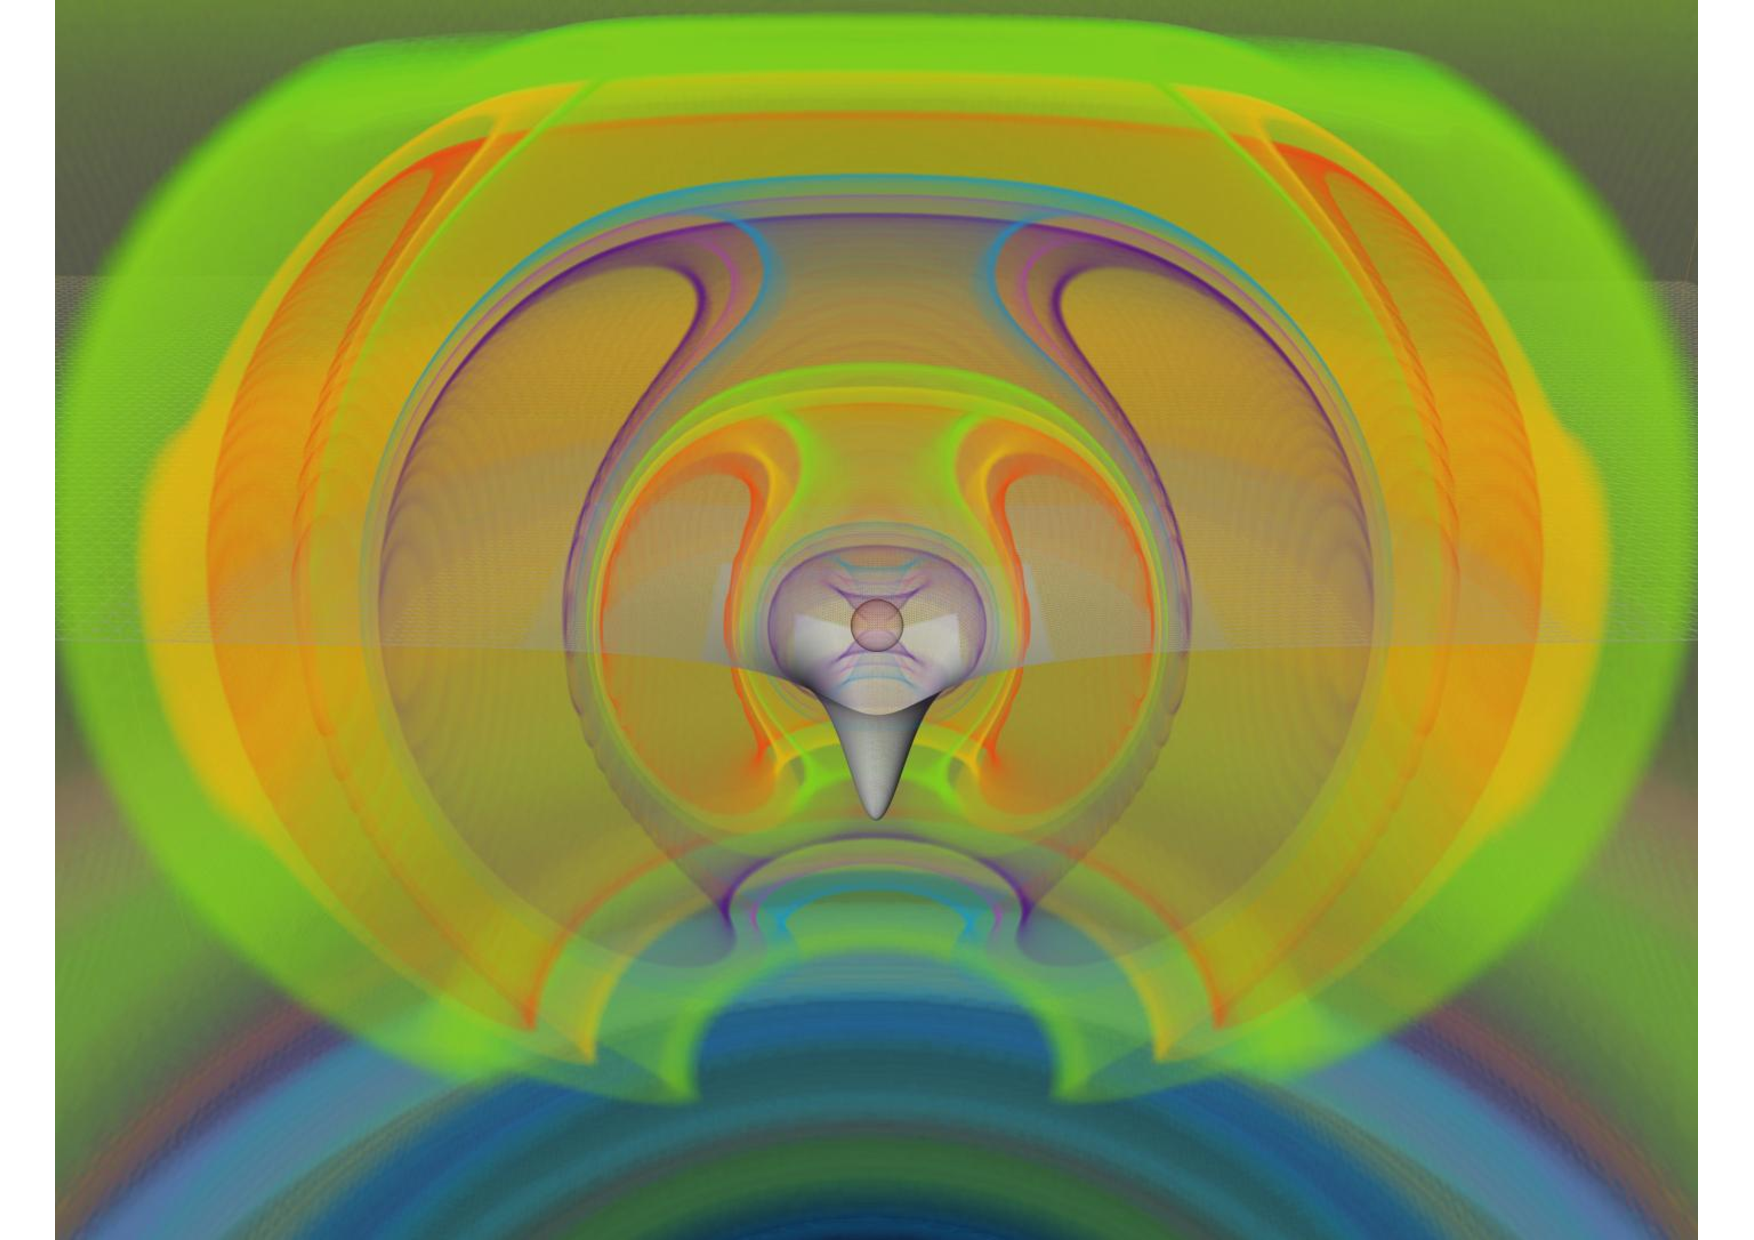
\includegraphics[width=0.88\linewidth,height=0.48\textheight,keepaspectratio]{../figs/pdf/en/fig-08-01.pdf}

% DOCX paragraph 1146
\caption{\emph{Numerical simulation of gravitational waves emitted by a perturbed black
hole. © R. Kaehler / LR.}}\label{fig:08-01}
\end{figure}

% DOCX paragraph 1148
Waves of this type are shown in Figure \ref{fig:08-01} and are the result of a numerical simulation.
The image details the gravitational waves produced in the first moments in which an
almost spherical neutron star collapses\index{gravitational!collapse} into a black hole that is not
yet perfectly spherically symmetric but has small perturbations shedding away.

% DOCX paragraph 1149
Putting aside the case of spherical symmetry\index{spherical symmetry} (which is an exception
as it is quite rare in nature to maintain a perfect spherical symmetry), it must be said
that, although gravitational waves are easy to generate, not all sources can produce
them efficiently enough or at frequencies that allow for experimental detection. We
return to these two aspects, the efficiency of emission and detection capability, later
on in this chapter. For the time being, let's concentrate instead on their effect on the
rest of spacetime when they propagate.

% DOCX paragraph 1150
To explain what happens when we interact with a gravitational wave, I will employ an
analogy with a type of wave closer to our lived experience: the water waves generated on
the perturbed surface of a lake. So, let's imagine we are on an inflatable mattress,
floating peacefully on the surface of a perfectly calm lake on a sunny and windless day.
At one point, we see someone jump from a boat in the distance. Their impact with the
water produces a perturbation that spreads outwards, with an essentially spherical front
and a decreasing amplitude, as the wavefront is distributed over an increasingly wider
surface. Once it reaches us, the perturbation is very small, and its wavelength (the
separation between successive crests in the wave) will be much greater than the size of
our inflatable mattress, which we can, therefore, consider as point-like (i.e., with
vanishingly small size). As a first approximation (or, in more mathematically precise
language, at first order in the perturbation), we can say that the waves will be
transverse, so our mattress will begin to oscillate with a periodic motion in the
vertical direction, i.e., perpendicular to the direction of propagation of the wave. In
this example, the water waves essentially do the job of transferring the kinetic energy
released by the person who jumped from the boat to the rest of the lake. Once the
wave-train (that is, the sequence of waves triggered by the jump) has passed completely,
the mattress will return to its initial position, at rest, and we can go back to
relaxing.\textsuperscript{\hyperlink{note:08-02}{2}}

% DOCX paragraph 1151
In analogy with the above description, we can perform a gedanken experiment. Imagine
that somewhere in the universe, gravitational waves are produced (through processes
described further on in the chapter) that reach us along a direction that is
perpendicular to the lake's surface, with a wavelength that is again larger (though not
by much) than the size of our mattress. Since gravitational waves are the transverse
type, the perturbation they propagate cannot be measured as a variation in the vertical
position of the mattress. Rather, they generate local changes in the value of the
curvature. More precisely, by changing the local curvature, gravitational
waves\index{gravitational waves!tidal forces} will generate ``tidal forces\index{tidal forces}'', which will
then induce variations in the position of objects not subjected to external forces. This
is similar to the tidal forces exerted by the Moon\index{Moon} on the Earth that
cause the displacement of liquid masses on our planet. Thus, the tidal fields that would
reach us in our gedanken experiment would induce deformations both on us and, above all,
the water around us. These deformations are of a very specific type, namely, of
\emph{quadrupolar} type, and consist of a ``compression'' in a given direction and a
``stretching'' in the orthogonal direction. As we will discuss later, these variations
will be periodic and emitted at the same frequency as the waves, which can either be
constant or vary over time.

% DOCX paragraph 1152
To better understand what we would be experiencing in our gedanken experiment, we can
rely on Figure \ref{fig:08-02}, which shows the quadrupolar deformations to which the
``\emph{Vitruvian Man''} by Leonardo Da Vinci\index{Leonardo Da Vinci} would be subject if
crossed by a gravitational wave. Fortunately for us, the gravitational
waves\index{gravitational waves!deformations} that reach the Earth are so weak that not only do they not
produce appreciable deformations in our bodies, but it is actually necessary to build
highly sensitive devices to detect them.

% DOCX paragraph 1153
\begin{figure}[htbp]
\centering
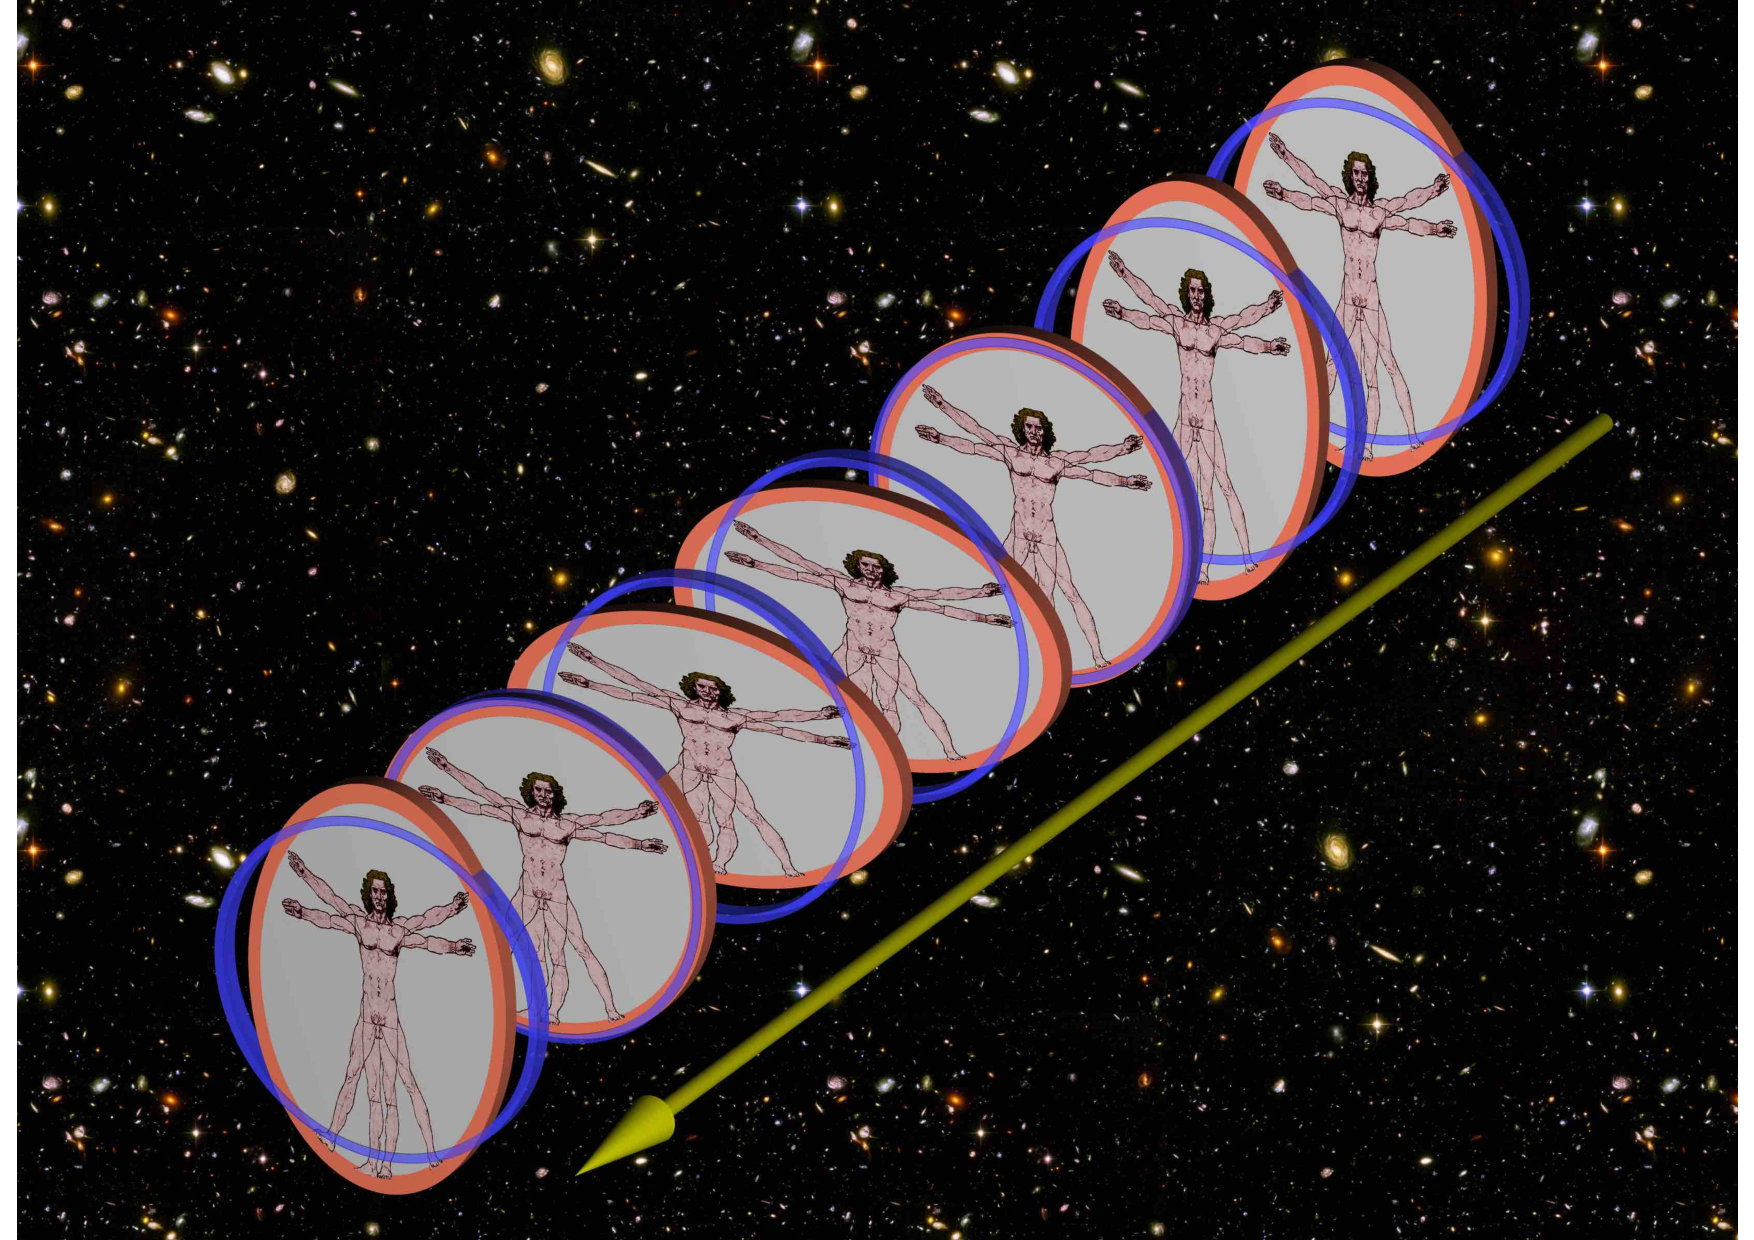
\includegraphics[width=0.88\linewidth,height=0.48\textheight,keepaspectratio]{../figs/pdf/en/fig-08-02.pdf}

% DOCX paragraph 1154
\caption{\emph{Quadrupolar deformation of the Vitruvian}\index{Leonardo da Vinci!Vitruvian man} \emph{Man
crossed by a gravitational wave. © M. Pössel (AEI) / LR.}}\label{fig:08-02}
\end{figure}

% DOCX paragraph 1155
It is important to comment here on an aspect that is not often given proper relevance.
In their mathematical formulation, the Einstein equations only behave like waves under
precise conditions: a vacuum\index{vacuum} spacetime, a weak field, and asymptotic
flatness\index{spacetime!flat}. These conditions are certainly not those present in the
vicinity of the source, where spacetime has a strong and very dynamic curvature.
However, these conditions are met from where we are, namely, at a great distance from
the sources and where these perturbations do behave like waves. For us, as distant
observers, curvature perturbations will therefore behave like waves and come in two
types, or two degrees, of \emph{linear
polarisation}\index{polarisation}\index{polarization!linear (plus)}. These are called ``\emph{plus
polarisation''} (indicated with a + symbol) and, identical to the plus polarisation but
rotated by 45 degrees, \emph{``cross polarisation''} \index{polarization!linear (cross)} (indicated with
a × symbol). To get a concrete idea of the difference between the two polarisations, we
can refer again to Figure \ref{fig:08-02}, which reports the effects of the plus polarisation. By
contrast, the cross polarisation would not compress and stretch the
\emph{Vitruvian}\index{Leonardo da Vinci!Vitruvian man} \emph{Man} in the direction between his head and
feet but, instead, would compress and stretch him along a diagonal direction to
this.\textsuperscript{\hyperlink{note:08-03}{3}}

% DOCX paragraph 1156
In general, the degree of polarisation of gravitational waves\index{gravitational waves!polarization (see polarization)}
reflects the properties of the source. Realistic astrophysical sources will produce
radiation containing a mixture of these polarisations, although it is possible to
generate gravitational\index{gravitational!radiation} radiation in a single polarisation under some
special conditions. Given these properties, let's now focus on why it is important to
study gravitational waves.

% DOCX paragraph 1159
\section{Gravitational And Electromagnetic Waves}\label{sec:08-comparison}

% DOCX paragraph 1161
It is often remarked that the combined detection of electromagnetic and gravitational
waves has marked the birth of \emph{multi-messenger}\index{astronomy!multi-messenger (gravitational-wave)}
\emph{gravitational-wave astronomy}, thus opening a new ``window'' on the universe. Both
of these statements are correct, although a little obscure, perhaps.

% DOCX paragraph 1162
Let's see what they signify and start by clarifying what ``multi-messenger'' astronomy
means. The formal definition is that it is a branch of astronomy in which scientific
knowledge is reached through different channels of information, called ``messengers''.
More specifically, in addition to the obvious electromagnetic channel (i.e., the light
emitted by celestial objects in the various bands), multi-messenger astronomy makes use
of other messengers, such as
neutrinos\index{astronomy!multi-messenger}\index{multi-messenger astronomy}\index{neutrino} (for instance, those
emitted in supernova explosions) or gravitational waves. In the latter case, it also
takes the name of \emph{multi-messenger gravitational-wave
astronomy}\index{astronomy!multi-messenger (gravitational-wave)}. The importance of multi-messenger astronomy is that, by
using more than one channel to obtain information and because the information contained
in the various channels can differ substantially, it has the potential of being much
``richer'' than traditional astronomy.

% DOCX paragraph 1163
To better illustrate what I mean, let me offer an example that I find fits very well and
is easy to understand. Imagine taking part in one of the many beautiful festivals that
characterise the Italian summer and that the program includes a late-night fireworks
display. Because you are passionate about fireworks, you have carefully chosen the best
spot to take in the sights. A position that offers an excellent and elevated view, far
enough away to observe the whole show but near enough to enjoy the full experience of
the blasting sounds. In essence, imagine sipping a glass of wine immersed in the warmth
of the summer night, enjoying an unforgettable fireworks display.

% DOCX paragraph 1164
Now, think about what this experience would be like if you were deprived of either sight
or hearing. If you could not discern the lights produced by the fireworks, you would
perceive the entire event as a sequence of explosions, some intense and low, others
weaker and more high-pitched, which would convey little of how spectacular the fireworks
were. If, on the other hand, you could not hear the sound produced by the fireworks, you
would find yourself watching a sequence of colourful and perhaps fascinating, but not
very engaging, images as if everything was taking place on a different planet. On
several occasions, I have happened to observe fireworks from a low-flying plane, and I
can guarantee you that it is much less exciting.

% DOCX paragraph 1165
This example illustrates how fireworks can be considered, for all practical purposes, as
a \emph{multi-messenger} phenomenon. This is because the information from fireworks
reaches us via both sound waves (the first messenger) and via electromagnetic waves (the
second messenger). Thanks to this analogy, you can fully and directly appreciate how
much richer and more informative multi-messenger astronomical observations can be when
compared to traditional ones. They allow us to investigate different aspects of a source
because they are conveyed by different messengers.

% DOCX paragraph 1166
Concentrating on how gravitational waves differ from other messengers helps us to
appreciate how gravitational waves represent a very different sort of messenger. The
vast majority of the information we receive about our universe comes to us through
electromagnetic waves. They cover a very broad spectrum\index{spectrum!electromagnetic}, from the
radio band to the gamma-ray band, but they have one property in common: they reveal
details about the \emph{thermodynamic} state\index{thermodynamic state} of the sources, namely,
their density and temperature. At the same time, the components of light (photons),
interact with the matter they encounter on their way to us, therefore experiencing
either absorption or additional emission. Indeed, an astronomical source could be
partially or completely eclipsed by the material interposed between us and it.
Gravitational waves are somewhat different because they transmit a tidal gravitational
field, so they are only loosely coupled to the forces that hold astronomical objects
together. As a result, they propagate almost undisturbed, providing us with information
on the global movements of the sources at frequencies very different from those of
electromagnetic waves; in this way, the information that gravitational waves convey is
necessarily different and thus complementary.

% DOCX paragraph 1167
The table below summarises the sometimes radical differences between electromagnetic
(EM) waves and gravitational waves (GWs) and the type of information they convey.
\index{gravitational waves!electromagnetic waves (vs)}\index{electromagnetic waves! gravitational waves (vs)}

% DOCX paragraph 1168
{\small
\setlength{\tabcolsep}{5pt}
\begin{longtable}{@{}>{\raggedright\arraybackslash}p{0.48\linewidth}>{\raggedright\arraybackslash}p{0.48\linewidth}@{}}
\toprule
% DOCX table after paragraph 1168, row 0, column 0
\textbf{EM Waves}
&
% DOCX table after paragraph 1168, row 0, column 1
\textbf{Gravitational Waves}
\\[6pt]
\midrule
% DOCX table after paragraph 1168, row 1, column 0
They are oscillations of electric and magnetic fields that propagate through spacetime.
&
% DOCX table after paragraph 1168, row 1, column 1
They are oscillations of the spacetime itself.
\\[6pt]
% DOCX table after paragraph 1168, row 2, column 0
The simplest are those relative to dipole\index{dipole!radiation} radiation, i.e., generated by an oscillating dipole\index{dipole!electric} (two opposite electric charges).
&
% DOCX table after paragraph 1168, row 2, column 1
The simplest are those relative to quadrupolar radiation\index{quadrupole!radiation}, i.e., generated by an oscillating mass quadrupole\index{quadrupole!mass} (a non-circular distribution of mass).
\\[6pt]
% DOCX table after paragraph 1168, row 3, column 0
They are almost always the result of the incoherent superposition of contributions from millions of electrons, atoms or molecules.
&
% DOCX table after paragraph 1168, row 3, column 1
They are produced by the coherent movement of large amounts of mass and energy, be they in the form of astronomical objects or energy condensations.
\\[6pt]
% DOCX table after paragraph 1168, row 4, column 0
They show us the details of the thermodynamic state\index{thermodynamic state} (temperature, density) of the sources that produce them.
&
% DOCX table after paragraph 1168, row 4, column 1
They show us the details of the dynamics and global properties (size, mass, and velocity) of large concentrations of mass/energy.
\\[6pt]
% DOCX table after paragraph 1168, row 5, column 0
Their wavelengths are very short compared to the size of the astronomical sources. Hence, it is possible to obtain ``images'' of the sources.
&
% DOCX table after paragraph 1168, row 5, column 1
Their wavelengths are often comparable to the size of the sources that produce them, if not greater. Hence, it is not possible to produce ``images'' of the sources.
\\[6pt]
% DOCX table after paragraph 1168, row 6, column 0
They suffer from absorption, diffusion and dispersion by the matter they encounter on their path.
&
% DOCX table after paragraph 1168, row 6, column 1
They propagate undisturbed, at the speed of light, through all types of materials.
\\[6pt]
% DOCX table after paragraph 1168, row 7, column 0
Those emitted by celestial objects have a spectrum\index{spectrum!electromagnetic} that is essentially independent of the mass of the source; for instance, the emissions from stellar and supermassive black holes are very similar.
&
% DOCX table after paragraph 1168, row 7, column 1
Those emitted by celestial objects have a spectrum\index{spectrum!gravitational wave} that depends on the mass of the source: the frequency of gravitational waves from stellar black holes is much higher than that from supermassive black holes.
\\[6pt]
% DOCX table after paragraph 1168, row 8, column 0
They have wavelengths shorter than the curvature radii of the objects they encounter as they propagate. For this reason, they experience gravitational lensing\index{gravitational!lensing}, i.e., distortion and amplification.
&
% DOCX table after paragraph 1168, row 8, column 1
They have wavelengths comparable if not greater than the curvature radii of the objects they encounter while propagating. For this reason, gravitational lensing is less pronounced and more difficult to measure.
\\[6pt]
\bottomrule
\end{longtable}
}


% DOCX paragraph 1170
After this synthetic comparison, I think it is clear that the possibility of observing
the same astrophysical phenomenon through the emission of gravitational waves and
electromagnetic waves represents a fantastic opportunity to multiply and amplify the
information collected. The first gravitational-wave event detected was
GW150914\index{GW150914}, whose name underlines that this is a gravitational-wave
(GW) event detected on September 14, 2015. The signal was produced by a binary system of
black holes and, for months after the detection, astronomers searched for an
``electromagnetic counterpart\index{electromagnetic counterpart}'', that is, for traces of a
corresponding electromagnetic emission in all possible bands, from gamma to radio.
Unfortunately, no electromagnetic\index{electromagnetic counterpart} counterpart was identified, and
this remains the case even now, several years later. Similar failures to detect an
electromagnetic counterpart have accompanied other gravitational-wave detections coming
from binary systems of black holes (at present, there are over 60). Fortunately, this
rather frustrating situation changed in 2017 with the event GW170817\index{GW170817}:
the merger of a binary system of neutron stars that gave us a fantastic display of
cosmic fireworks. We will talk about this event soon.

% DOCX paragraph 1173
\section{How Do We Detect Gravitational Waves?}\label{sec:08-detectors}

% DOCX paragraph 1175
We have seen that the production of gravitational waves is by no means a rare or complex
phenomenon, quite the contrary. What makes them so unusual in our experience is that the
amplitude of the gravitational waves we usually receive on Earth is not large enough to
be measured by an experimental device. To understand why, we must first remember that
the propagation of a gravitational wave manifests itself through tidal fields that
induce a variation in the size of the objects encountered. Shortly, we will discuss in
more detail what produces gravitational waves with an amplitude that allows us to reveal
them, but I can mention here that, even considering the strongest astrophysical sources
imaginable (a binary system of black holes) and taking into account the typical
distances of these sources, the amplitude ``\emph{h}'' at which their gravitational
waves reach us is of the order of only \emph{h} \(\simeq \ \)10\textsuperscript{--21}, a
number so small it is equivalent to one part in 1,000,000,000,000,000,000,000. It is
hard to imagine the precision required to measure such a small number, but it is as if
we wanted to measure a length equal to one billionth of the diameter of an atom, or,
equivalently, the distance between the Earth and Proxima Centauri\index{Proxima Centauri},
with an accuracy of 40 microns!

% DOCX paragraph 1176
This precision would seem impossible to achieve in practice. Yet, after decades of
research and continuous improvements, modern gravitational-wave detectors, such as LIGO
or Virgo \index{LIGO}\index{Virgo}, are now able to operate at this level
of precision. So, ``How do they achieve similar results?\emph{''.}

% DOCX paragraph 1177
The answer is found in the use of a technique we discussed in the previous chapter:
interferometry. In the case of gravitational-wave detectors\index{gravitational waves!detectors}, the
basic operation involves a relatively simple device, based on an experiment conducted at
the end of the nineteenth century by the American physicists Albert
Michelson\index{Michelson!Albert} and Edward Morley \index{Morley!Edward}, aimed at measuring
the motion of the Earth through a hypothetical medium, the
``aether\index{aether}''. Unfortunately, the experiment showed that this medium
does not exist. However, the very ingenious experimental device, known as a
\emph{Michelson-Morley
interferometer}\index{Michelson!interferometer}\index{Morley!interferometer}\index{interferometer!Michelson-Morley}, remained and
was later adopted for gravitational- wave detection.

% DOCX paragraph 1178
Figure \ref{fig:08-03} shows a simplified diagram of such an interferometer\index{interferometer}. As
you can see, a light source as coherent and stable as possible produces a beam of light
(today, powerful lasers are used, but at the end of the nineteenth century, technology
was more rudimentary), this beam of light is collected by a semi-reflective
mirror\index{mirror!semi-reflecting}\index{gravitational-wave detector!mirrors}. These are mirrors capable of reflecting
only a part of the incident light, letting another part pass, just like those in police
stations used to observe an interview room without being seen. Regarding
gravitational-wave interferometers, very sophisticated mirrors are used to reflect
precisely 50 percent of the light, allowing the remaining 50 percent to pass through.
Furthermore, suppose the mirror is placed at 45 degrees to the incident beam, as shown
in the figure. In that case, it ``splits'' the beam in two (in fact, they are also
called ``beam splitters\emph{''})\index{gravitational-wave detector!beam splitter}, letting light propagate in two
orthogonal directions, which represent the so-called ``\emph{arms}'' of the
interferometer (the arms can be made virtually longer by adding a new mirror and
creating what is called a Fabry-Pérot cavity).

% DOCX paragraph 1180
\begin{figure}[htbp]
\centering
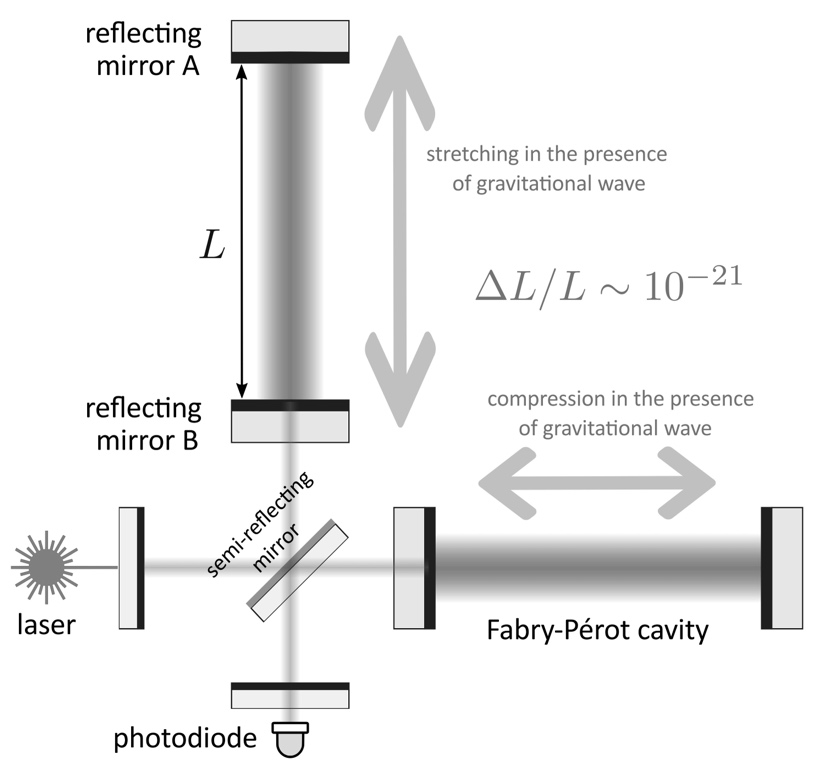
\includegraphics[width=0.88\linewidth,height=0.48\textheight,keepaspectratio]{../figs/source/en/fig-08-03.jpeg}

% DOCX paragraph 1182
\caption{\emph{Scheme of an interferometric gravitational-wave detector.}}\label{fig:08-03}
\end{figure}

% DOCX paragraph 1184
In the original experiment of 1887, the length of the two arms was of the order of about
ten metres, decidedly insufficient to measure gravitational waves. Since the relative
variation of the arms induced by a gravitational wave (normally indicated as
\emph{ΔL/L}) is equal to the amplitude of the wave itself (which we have seen to be
\emph{h} ≃ 10\textsuperscript{--21}), current technology only allows measurements to be
made if the length of the interferometer arms, \emph{L}, is of the order of a few
kilometres. For this reason, the LIGO\index{gravitational-wave detector!LIGO} interferometric detectors (one
located in Livingston, Louisiana and the other in Hanford, Washington State) have arms
of four kilometres. Whereas the Virgo\index{Virgo} \index{gravitational-wave detector!Virgo}detector in
Cascina, near Pisa, has slightly shorter arms of three kilometres.

% DOCX paragraph 1185
The beam splitter divides the initial laser beam into the two orthogonal beams that
travel along the arms until they reach the first reflecting mirror\index{mirror!reflecting}
suspended with thin silicon wires (``mirror A'' on the vertical arm), which reflects the
incoming beams. As you can imagine, these mirrors are more elaborate than ones we are
used to; in fact, they are small technological marvels. In addition to being nearly
twenty centimetres thick and weighing several tens of kilos, their surface is so smooth
that their roughness is of the order of a nanometre, that is, a few billionths of a
metre. Furthermore, if the mirrors in our house have a reflectivity of between 80 and 90
percent, theirs is greater than 99.9999 percent. In other words, only one
photon\index{photon} in a million is absorbed rather than reflected.

% DOCX paragraph 1186
Once reflected by these astonishing instruments, the laser beams return, join, pass
again through the beam splitter, and interact at an interferometric level with a very
light-sensitive electronic device called the \index{gravitational-wave detector!photodiode} ``\emph{photodiode''}.
In general, in the absence of gravitational
radiation\index{gravitational!radiation}\index{radiation!gravitational}, the interferometer can be ``tuned'' so
that, upon their return to the beam splitter, the two light beams are either perfectly
\emph{``in phase''} or ``\emph{in} \emph{phase} \emph{opposition''}. In this way, they
can produce a constructive interference\index{interference} when they are in phase (their
light adds up) or destructive interference when they are in phase opposition (their
light cancels). For practical purposes, it is convenient that the interference measured
by the photodiode is the destructive one and the whole interferometer is, in fact, tuned
so that the photodiode is on the ``dark fringe''.

% DOCX paragraph 1187
The passage of a gravitational wave propagating in a direction orthogonal to the plane
containing the two arms would produce a tidal distortion and thus a relative variation
of the arm lengths. In turn, this would produce a phase shift between the paths
travelled by the light in the two arms and hence a variation of the
interference\index{interference} at the photodiode, which would no longer be synchronised
on a dark fringe. The greater the amplitude of the gravitational wave, the greater the
distortion of the arms, and therefore the phase shift in the light recombined at the
photodiode.

% DOCX paragraph 1188
I have just described, carelessly leaving out some important details, the basic
functioning of a classic Michelson-Morley interferometric experiment. However, if we
managed to build an interferometer of this type, with four-kilometre long arms, we would
not detect any gravitational waves! This is because the deformations they produce, and
therefore the amplitude of our \emph{signal,} would still be too small compared to those
that are inevitably produced by the environment, which represent so-called
\emph{noise}\index{noise}. Since we cannot change the amplitude of the signal,
which is entirely and solely determined by the properties of the source, our only hope
of detection comes from reducing the noise as much as possible. For us to do this, it is
necessary to resort to a whole series of experimental measures aimed at reducing the
noise level below that of the signal, i.e., increasing the
signal-to-noise\index{signal-to-noise ratio}\index{noise!signal-to-noise ratio} ratio. It is similar to being in a
room and hearing a tune that you recognise but can't place because the noise made by
other people in the room prevents you from clearly distinguishing the notes. Not being
able to increase the music volume, your only option is to reduce the noise, so you ask
the others in the room to be quiet for a moment.

% DOCX paragraph 1189
Numerous techniques have been developed over the past 40 years to break down the various
sources of noise that affect modern gravitational-wave detectors. As interesting and
ingenious as these techniques are, discussing them would take more time than we have
left on this last part of our journey. What matters here is to underline that detectors
such as LIGO and Virgo represent the result of the joint work of thousands of people
and, like EHTC radio-telescopes\index{radio-telescope!EHT} or the accelerators at
CERN\index{CERN}, they must be seen as the apical expression of human
technological capabilities. Ultimately, these detectors represent the only tool
available for detecting the sources of gravitational waves, which we will discuss in the
next section.

% DOCX paragraph 1192
\section{Who Makes The Waves?}\label{sec:08-sources}

% DOCX paragraph 1194
The title of this section is intentionally incomplete. By now, you know that any
non-spherical variation in time of a concentration of
mass/energy\index{energy!mass equivalence}\index{mass!energy equivalence} produces gravitational waves.
Therefore, the complete but obviously too long title should have been: ``What are the
sources\index{gravitational waves!sources} of gravitational waves that can be detected?''. The answer to
this question is rather simple: all sources that are sufficiently ``powerful'', that is,
able to release sufficiently large quantities of energy in the form of gravitational
waves.

% DOCX paragraph 1195
It has been quite some time since I last proposed an equation, and I definitely do not
want you to get out of the habit of reading them~... For this reason, I give below an
approximate but compact expression for the luminosity\index{ luminosity!gravitational wave}, i.e., the
amount of energy per unit of time, of a gravitational-wave source. This famous
expression, also known as the ``\emph{quadrupole}\index{quadrupole!formula} \emph{formula}'',
tells us that the luminosity of a source of gravitational waves is simply given by the
following basic properties of the source (note I intentionally ignore any numerical
factor):

% DOCX paragraph 1197
\begin{equation}\label{eq:08-01}
L_{GW} \simeq \textcolor{gray}{Gc}\left( \frac{M}{R} \right)^{2}\left( \frac{v}{v} \right)^{6} \simeq \textcolor{gray}{\frac{c^{5}}{G}}\left( \frac{r_{s}}{R} \right)^{2}\left( \frac{v}{v} \right)^{6}
\end{equation}

% DOCX paragraph 1199
In the formula, \emph{M} is the mass of the source, \emph{R} is its characteristic size
(for example, the radius if we think of a star or a black hole), and \emph{v} is the
average speed at which it moves. As usual, I have greyed out the parts related to
constants, which do not play an important role in understanding the equation.

% DOCX paragraph 1200
When looking a bit more carefully at Equation \eqref{eq:08-01}, we can see that it contains three
terms: the first one on the left is simply the definition of luminosity; the second one
in the middle expresses the luminosity in terms of mass and speed; the last one on the
right instead uses a quantity that we saw in chapter 6, namely the Schwarzschild radius:
\emph{r\textsubscript{s}=2GM/c\textsuperscript{2 }}(recall Equation (6.1)). First, let's
focus on the piece in the middle of the formula \eqref{eq:08-01}. It tells us that the luminosity
is proportional to a quantity we have encountered several times during our journey, that
is, the compactness of the source \emph{M/R} and, in particular, its square.
Furthermore, the luminosity is also proportional to the speed of the source (expressed
in terms of the speed of light) and, in particular, to its sixth power.

% DOCX paragraph 1201
In its simplicity, Equation \eqref{eq:08-01} sheds light on many details that had perhaps remained
obscure until now. Since most astrophysical structures have very small compactness and
move at much slower speeds than that of light, their luminosity in terms of
gravitational waves emitted is inevitably minute. Let's take the concrete example of the
Sun. We have seen its compactn\index{compactness!Sun}ess is of the order of \emph{M/R} ≃
10\textsuperscript{--6} (recall Equation (4.3)) and that it darts through our galaxy at
a speed of around 800,000 kilometres per hour, a few thousandths of the speed of light.
Therefore, we can use Equation \eqref{eq:08-01} to calculate its gravitational-wave luminosity and
find that it is: \emph{L\textsubscript{GW}} ≃ 10\textsuperscript{8} Watt ≃
10\textsuperscript{--18} \emph{L\textsubscript{EM}}. In other words, the Sun's
``luminosity'' \index{ luminosity!Sun} in gravitational waves is less than one billionth of
a billionth of that emitted in the form of electromagnetic radiation\index{radiation!electromagnetic}.
And if this is true for our star, which still moves at a considerable speed and has a
certain compactness, you can easily guess how futile it is to try to generate detectable
gravitational waves here on Earth. For example, imagine that you want to build a
gravitational-wave source by using a mass of one tonne (1,000 kilograms) and a size of
one metre that moves at one hundred kilometres per hour. This could be, for instance, a
small but heavy car travelling on a closed circular circuit with a radius of one
kilometre. In this case, the amplitude of the gravitational waves produced would be as
small as \emph{h} ≃ 10\textsuperscript{--43}: a few millionths of a billionth of a
billionth of what the best detectors can measure today. I don't think it is worth trying
this out~\ldots{}

% DOCX paragraph 1202
Instead, let's now focus on the third piece in Equation \eqref{eq:08-01}. It tells us that the
gravitational-wave luminosity\index{ luminosity!gravitational wave} is greatest when an object has
dimensions comparable to its Schwarzschild radius and moves at a speed very close to
that of light. This makes perfect sense and explains why the first measured signal of
gravitational waves was that produced by a binary system of black holes; they are very
simply the most powerful sources imaginable. By definition, the components of the system
have a size that is \emph{exactly} equal to the Schwarzschild radius, and they move at
about 2/3 of the speed of light in the final stages of their inspiralling
orbits\index{orbit!inspiralling}. Furthermore, since they are part of a binary system, they
offer the greatest possible deviation from spherical symmetry\index{spherical symmetry}.

% DOCX paragraph 1203
In summary, Equation \eqref{eq:08-01} gives us a very clear message: if we want to have any hope of
detecting gravitational waves with present interferometric detectors, we must collect
the signal from objects that are extremely compact (i.e., with \emph{M}≃\emph{R}), have
dimensions comparable with the Schwarzschild radius (i.e., with
\emph{R}≃\emph{r\textsubscript{S}}), and that move at a speed close to that of light
(i.e., with \emph{v}≃\emph{c}). Gravitational waves emitted by sources of this type, and
placed at a distance of a few hundred megaparsecs, will reach Earth with an amplitude
\emph{h}≃10\textsuperscript{--21} that, although at the limit of our instruments'
sensitivity, can in principle be measured.

% DOCX paragraph 1206
\section{The Zoology Of Gravitational-wave Sources}\label{sec:08-zoology}

% DOCX paragraph 1208
Now that we know what it takes to produce strong emissions of gravitational
waves\index{gravitational waves!waves}, it is useful to classify the various gravitational-wave
signals we could detect based on the sources that produce them. As we will see,
different sources will imprint their specific properties on the characteristics of the
signals, which will vary in terms of amplitude, frequency, and duration in time.

% DOCX paragraph 1210
\emph{Impulsive signals.} These are very short signals, i.e., of the order of tens of
milliseconds or less, and can be produced by different sources. For example, signals of
this type are expected in association with supernova\index{supernova} explosions or
the gravitational collapse leading to the formation of either a neutron star (as with
supernovae) or a black hole. Since these are short and evanescent signals, their
``spectral properties'' (the window in frequency in which the signal appears and the
amplitude at the various frequencies) are not well defined. In general, however, we are
looking at signals at high or very high frequencies, starting from a few hundred hertz
and going up to several kilohertz. Given the sensitivity of current detectors and the
signal from a supernova being rather weak, impulsive signals of this type are mostly
expected from our ``neighbourhood'', that is, within our galaxy. Although very common
and observable electromagnetically, even at the greatest distances, extragalactic
supernova explosions would be too far away and not be ``visible'' by gravitational-wave
detectors. Studies of the rate of supernova explosions within our galaxy indicate that
we should expect one supernova explosion every 30 or 40 years. Hence, it is not
surprising that LIGO/Virgo has not yet measured such signals, although we are all
anxiously awaiting the first one!

% DOCX paragraph 1211
Precisely because of their ``impulsive'' nature, signals of this type could be linked to
sources that have been predicted but never observed so far, such as cosmic strings,
which are relics of phase transitions in the early universe. Furthermore, should a
wholly new and unexpected source exist that no theory has yet predicted, it is very
likely that the corresponding signal will be of the impulsive type. For this reason,
measuring the first impulsive signal would be a doubly exciting event!

% DOCX paragraph 1212
{\setlength{\spaceskip}{\fontdimen2\font plus 2pt minus \fontdimen4\font}
\emph{Periodic signals.} These are signals from sources that produce a
gravitational-wave signal at a single precise frequency or at a limited set of very
specific frequencies. Notably, the amplitude of the signals and the corresponding
frequencies are expected to remain constant over periods of tens if not hundreds of
years. Potential sources of periodic gravitational waves are clearly pulsars, objects
already encountered in Chapter 5 that we know emit a beam of electromagnetic
radiation\index{radiation!electromagnetic} that hits us like the light from a
lighthouse\index{lighthouse} beacon. These rotating neutron stars can deviate from
perfect axial symmetry due to small deformations on their surface (our ``mountains'' in
Chapter 5) \index{neutron star!mountains}, produced when the neutron star's crust solidifies in the
rapid cooling process after its birth. Alternatively, the deformations can be present in
the stellar core if it is a crystal, or they can be induced by the presence of a strong
magnetic field, which, through magnetic tension, gives rise to non-axisymmetric
stresses.

\par}

% DOCX paragraph 1213
In essence, given the great compactness and rapid rotation of neutron stars, it is
sufficient that a slight asymmetry is present for it to generate a gravitational-wave
signal that is detectable within our galaxy. You may think that this type of signal
should be easy to detect. Unfortunately, it is quite the opposite for a number of
reasons. Although the emission occurs at a precise frequency, the frequency is unknown.
Also, the signal is extremely weak, and the
signal-to-noise\index{noise!signal-to-noise ratio}\index{signal-to-noise ratio} ratio can even drop below unity.
It is, therefore, only through observations lasting weeks or months that it is
potentially possible to ``extract'' this weak signal from the sea of detector noise in
which it is immersed. The observation campaigns carried out so far by LIGO and Virgo
have not yet revealed any source of periodic gravitational waves. However, they have
provided tight constraints on the ``height'' of the mountains possibly present on the
surface of some targeted neutron stars, which cannot exceed one millimetre and, in many
cases, are well below a tenth of a millimetre.

% DOCX paragraph 1214
\emph{Stochastic signals.} This type of signal is markedly different from those
described so far in that the sources responsible for it are not ``resolved''
individually. In other words, it is possible to associate the measured signal only to a
collection (often very large) of sources that cannot be distinguished individually by
the instruments. Furthermore, each of these sources is too faint to be detected in
isolation, but when taken together, they become measurable. To better understand how
this is possible, let me use a very simple but effective example. Take the image of a
distant galaxy that you can already see with a small telescope. It will appear as a
small nebula because the light that reaches you is the combination of the light of tens,
if not hundreds, of billions of stars, which, of course, you cannot distinguish
individually. Taken in isolation, none of the stars contributing to the image would
actually be visible. However, once put together, their emission combines positively and
allows you to see the distant galaxy. The same logic applies to sources of gravitational
waves that are not resolved individually, but that can be detected by combining the weak
signals that all the sources produce.

% DOCX paragraph 1215
There are several classes of sources of stochastic signals. One of these is the
stochastic \emph{``}background\index{gravitational waves!background}\emph{''} of astrophysical origin
produced by a large number of binary systems of white dwarfs\index{white dwarfs} or brown
dwarfs\index{brown dwarfs}. These types of objects represent stars in the final stages of
their life, and there are billions of them in our galaxy alone. Brown and white dwarfs
are more compact than ordinary stars but also much less compact than neutron stars.
Apart from those binaries that are very close and well-known, the signal they produce is
too weak to be identified individually. The simple reason is that they are not compact
enough and do not move in their orbits at sufficiently high speeds (recall Equation
\eqref{eq:08-01}). However, when millions of these sources are ``switched on'' and emitting
gravitational waves, the signals are, in fact, detectable as an indistinct background,
as long as the observation time is long enough. The typical period of the gravitational
waves produced by these sources is about one hour, a frequency too low to be measured by
interferometers such as LIGO or Virgo. However, they will certainly be ``visible'' by
the LISA\index{gravitational-wave detector!LIGO}\index{LISA} space interferometer, which is due to be
launched around 2035, and for which they will represent a source of
noise\index{noise}.

% DOCX paragraph 1216
Another type of stochastic background is of cosmological origin and could have been
generated soon after the Big Bang due to very small but nonzero perturbations in the
density distribution across the universe. These cosmological gravitational waves are at
extremely low frequencies, but a part of them should have a signal with periods of tens
of days and, therefore, potentially be accessible to LISA. Since they were emitted only
10\textsuperscript{-43} seconds after the Big Bang, measuring them directly or
indirectly (through the ``footprint'' they may have left on the cosmic
microwave\index{cosmic microwave background} background\textsuperscript{\hyperlink{note:08-04}{4}}) would be extremely valuable.
It would allow us to obtain information on the physical conditions of our universe in
the very first moments of its life.

% DOCX paragraph 1217
\emph{Signals from binary systems.} These are the gravitational signals ``par
excellence'', as they are among the strongest possible and the only ones detected so
far, either directly or indirectly. Several aspects of this type of signal merit
detailed discussion, and I will do this in the following pages. Here though, I will
limit myself to remarking on the bare minimum.

% DOCX paragraph 1218
In particular, I will call to mind that there are two classes of astrophysical objects
that are undisputed champions of compactness\index{compactness!neutron star}\index{compactness!black hole},
neutron stars and black holes. Hence, they are potentially strong sources of
gravitational waves just because they are so compact. To this significant advantage, you
can add that it is relatively common to find these compact objects in binary systems
composed of two black holes, two neutron stars, or in a ``mixed'' configuration. This
characteristic is doubly important as it gives the source a considerable deviation from
a spherical symmetry\index{spherical symmetry}, in fact, the greatest possible. At the same
time, it allows the components of the binary system to reach speeds close to that of
light when they are about to merge. Combining these factors, and bearing in mind the
Equation \eqref{eq:08-01}, it is not difficult to conclude that those generated by binary systems
of black holes and neutron stars\index{neutron star!gravitational waves (see)} are the strongest gravitational wave
signals.

% DOCX paragraph 1219
As an effective way of concluding this section on the zoology of gravitational-wave
sources, Figure \ref{fig:08-04} provides an overview of what we have discussed so far. The position
of each source on the horizontal axis serves to give an idea of the ``characteristic
frequency'' (or period) at which the gravitational wave is emitted. This, therefore,
allows us to compare sources with periods of days (i.e., with frequencies of tens of
millionths of a hertz, as for binary systems of supermassive black holes) or of tens of
milliseconds, and even less (i.e., with frequencies of hundreds or thousands of hertz,
as for binary systems of neutron stars). The vertical position of each source, on the
other hand, gives a rough idea of the ``characteristic amplitude'' of the gravitational
waves. Finally, the lines in the graph represent the sensitivity curves of
interferometric detectors such as LIGO/Virgo or the future LISA\index{LISA}
spatial interferometer and inform us how well these sources can be detected.

% DOCX paragraph 1221
\begin{figure}[htbp]
\centering
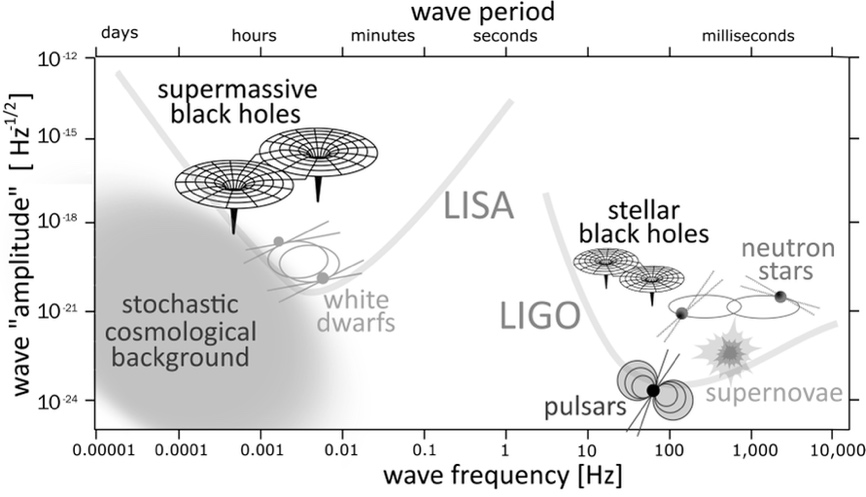
\includegraphics[width=0.88\linewidth,height=0.48\textheight,keepaspectratio]{../figs/source/en/fig-08-04.jpeg}

% DOCX paragraph 1223
\caption{\emph{The various sources of gravitational waves identifiable by detectors such
as LIGO/Virgo or LISA}\index{LISA}\emph{.}}\label{fig:08-04}
\end{figure}

% DOCX paragraph 1224
Note that the sources shown are not all at the same distance from us. On the contrary,
the reported characteristic amplitude refers to sources at the limit of the
\emph{observational horizon}\index{observational!horizon}, that is to say, the volume of the
universe within which each of the sources can be observed. This horizon will be limited
to our galaxy (i.e., to a distance of about one hundred kiloparsecs from us) in the case
of the gravitational-wave signal from a supernova explosion. However, it will be of tens
of megaparsecs in the case of binary systems of neutron stars and even hundreds of
megaparsecs in the case of binary systems of stellar black holes. Finally, the
observational horizon of LISA\index{LISA} will include a large part of the
observable universe since it will essentially ``see'', albeit with different
intensities, all of the binary systems of supermassive black holes that enter its
frequency range.

% DOCX paragraph 1225
Figure \ref{fig:08-04}, therefore, brings together every source that we realistically expect to be
able to observe in terms of gravitational waves. In reality, deep down, each of us
working in this field hopes that at some point a signal will be measured that does not
correspond to any of those reported in Figure \ref{fig:08-04}. Detecting such an unexpected source
would indicate something is wrong in our theoretical description of gravitational-wave
sources. At the same time, however, it would give us an excellent reason to question
everything!

% DOCX paragraph 1228
\section{The Difficult Life Of A Couple}\label{sec:08-couple}

% DOCX paragraph 1230
We tend to associate the first detection of gravitational waves from a binary system
with GW150914\index{GW150914} (the first event measured in 2015 by LIGO) and
corresponding to the merger of a binary system of black holes. However, in reality,
thanks to work that began 20 years earlier, it was already evident in the 1990s that
Einstein was right, and gravitational waves are produced by a binary system of compact
objects.

% DOCX paragraph 1231
But let's proceed in order. We have seen that the first pulsar was discovered in 1967
and that, since then, neutron stars have been observed either as isolated pulsars or in
binary systems, where the neutron star emits X-ray\index{X-ray!radiation} radiation from the
accretion of matter coming from the companion star. Since more than 50 percent (and
possibly as much as 85 percent) of stars are not isolated but gravitationally
bound\index{gravitationally!bound} in binary (or triple) systems, it did not take long to conclude
that two neutron stars\index{neutron star!binary (see)} could be present in a binary system.

% DOCX paragraph 1232
Probably inspired by considerations of this kind, in the early 1970s, the American
astronomers Russell Hulse\index{Hulse, Russell} and Joseph Taylor\index{Taylor, Joseph}
started a systematic campaign of observations of pulsars potentially belonging to a
binary system. They used the Arecibo radio-telescope in Puerto Rico, made up of 38,000
aluminium panels housed in a natural cavity creating a radio-reflecting dish nearly
three hundred metres in diameter. They soon concentrated their observations on the
pulsar PSR B1913+16\index{PSR B1913+16}, discovered in 1974.

% DOCX paragraph 1233
On paper, this pulsar is nothing peculiar, with a mass of 1.44 solar masses and a
rotation period of about 60 milliseconds, which means that it rotates on itself 17 times
per second. There was, however, something anomalous in its radio emission, something not
seen with any of the pulsars known at that time. In order to explain this singular
behaviour, it had to be acknowledged that the star orbited a companion; the problem was
that such a companion should have been visible, but it was not. However, if the
companion was also a neutron star, this would explain the observations quite well. This
was how Hulse and Taylor came to discover the first binary system of neutron stars, also
known as the \emph{Hulse-Taylor binary pulsar}, since it is a binary containing two
neutron stars, one of which is a pulsar.

% DOCX paragraph 1234
Today, thanks to the enormous precision of radio-astronomical observations of pulsars,
we know PSR B1913+16\index{PSR B1913+16} exceptionally well. For example, we know that
the masses of the two neutron stars are very similar (the primary has 1.441 solar
masses, the secondary 1.387) and that the orbital period is 7.75 hours. The orbits are
elliptic, so the two stars orbit the common centre of mass, and their separation varies
continuously, reaching about 1.1 solar radii (746,600 km) at the point of minimum
separation (periastron\index{periastron}) and about 4.8 solar radii (3,153,600 km) at
the point of maximum separation (apoastron\index{apoastron}). Given the masses
involved and the high orbital speeds reached by the stars, the binary pulsar PSR
B1913+16 represents a system in which relativistic\index{relativistic!effect} effects are
amplified and therefore easier to measure. For instance, just like
Mercury\index{Mercury!orbit}'s orbit, that of the pulsar is also not closed but
experiences a change of the periastron (recall Figure 2.1). The crucial difference is
that the periastron of PSR B1913+16 advances by 4.2 degrees every year, while
Mercury's\index{Mercury!periastron} advances by only 0.4297 arcseconds per year. In other
words, the orbit of PSR B1913+16 varies in a single day as much as Mercury's does in one
century!

% DOCX paragraph 1235
The most important relativistic\index{relativistic!effect} effect in PSR
B1913+16\index{PSR B1913+16} is linked to the emission of gravitational waves, which
reduces the energy and angular momentum of the binary and forces the two stars to get
closer. In particular, their separation is reduced by three millimetres after each
period, so, over one year, it has decreased by about 3.5 metres. In absolute terms, the
loss of energy from a binary system such as that of PSR B1913+16 is enormous;
furthermore, this system is actually in our galaxy and not very far from us at 21,000
light years away. Yet, the amplitude of the gravitational waves produced by the binary
is too small for detectors, such as LIGO and Virgo, designed for systems at much higher
frequencies (see Figure \ref{fig:08-04}). Nevertheless, the emission of gravitational waves is
``visible'' through the effects it produces on the evolution of the pulsar's orbit and,
in particular, on the change of the time at which PSR B1913+16 should reach its
periastron\index{periastron}.

% DOCX paragraph 1236
Figure \ref{fig:08-05} shows the advance in time of the binary's arrival at the
periastron\index{periastron} as a function of the year the observations were carried
out. That is to say, the decrease in the time required for the pulsar to complete a full
orbit is reported with points and error bars in Figure \ref{fig:08-05}. Note that the reported data
summarises observations carried out over 30 years and clearly illustrates how the
orbital period of PSR B1913+16\index{PSR B1913+16} (approximately seven hours and 45
minutes) has decreased by almost 40 seconds over such a timescale. Moreover, when
expressed in terms of the separation between the two neutron stars\index{neutron star!binary (see)},
this has decreased by 105 metres!

% DOCX paragraph 1237
\begin{figure}[htbp]
\centering
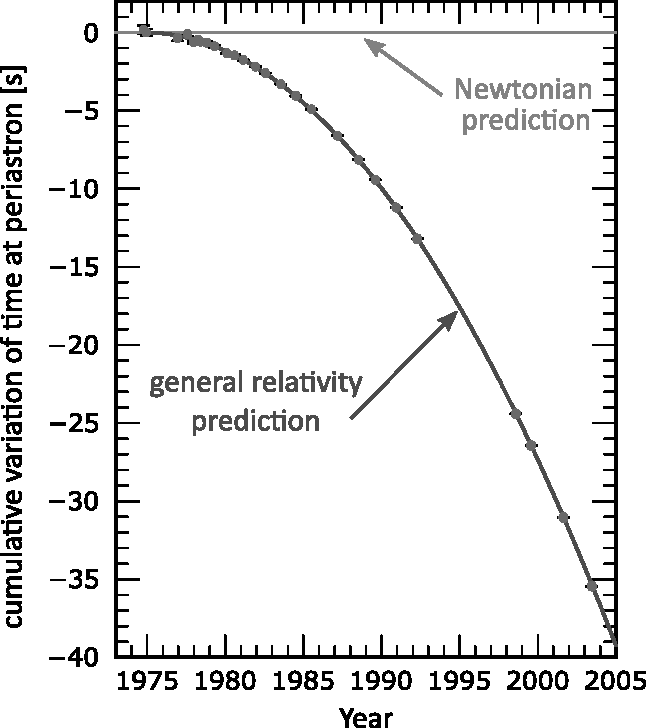
\includegraphics[width=0.88\linewidth,height=0.48\textheight,keepaspectratio]{../figs/pdf/en/fig-08-05.pdf}

% DOCX paragraph 1239
\caption{\emph{Observations of the decay of the orbit of PSR
B1913+16}\index{PSR B1913+16} \emph{in terms of the advance of the
periastron}\index{periastron} \emph{time. © data by J. M. Weisberg and J. H. Taylor,
ASP Conf. Series, 328, 25 (2005).}}\label{fig:08-05}
\end{figure}

% DOCX paragraph 1241
This example highlights an important feature of binary systems and the title of this
section. Independent of their nature and mass, a couple of astrophysical objects that
are gravitationally bound\index{gravitationally!bound} in a binary system must,
eventually~\ldots~``collide''! In the vast majority of cases, the timescales for this
process are simply enormous, much longer than the age of the universe. For example, in
the case of the Earth-Moon\index{Moon} binary system, the merger is expected in
65 billion years and does not represent an urgent source of concern. On the other hand,
the timescales for binary systems of compact objects are much reduced and of the order
of a few tens of millions of years. This shorter window allows us to ``witness'' the
occurrence of such collisions.

% DOCX paragraph 1242
The solid lines in Figure \ref{fig:08-05} refer instead to the theoretical predictions according to
Newton's theory of gravity (just a horizontal line since there can be no variation for a
closed orbit) and according to Einstein's general relativity. In the latter case, the
curve is not horizontal because the orbit must change (shrink) due to the emission of
gravitational waves. It is remarkable how perfectly the experimental measurements fit
with the theoretical curve predicted by general relativity. For this reason, the
observation of PSR B1913+16\index{PSR B1913+16} represents the first \emph{indirect}
proof of the existence of gravitational waves. Following the measurement of this
process, Hulse and Taylor were awarded the Nobel Prize in Physics in 1993. Obviously,
this result does not detract from the work of LIGO, whose observation of
GW150914\index{GW150914} has provided the first \emph{direct} proof of the existence
of gravitational waves.

% DOCX paragraph 1243
If what I've just told you about the remarkable properties of PSR
B1913+16\index{PSR B1913+16} blows your mind and pushes you to imagine two stars with a
diameter of about 25 kilometres orbiting one another at millions of kilometres per hour,
then you had better get prepared --- there is, in fact, a binary pulsar system that is
even more extreme! In 2003, using the radio-telescope at the Parkes\index{radio-telescope!Parkes Observatory}
Observatory in Australia, an international team, coordinated by the Italian astronomer
Marta Burgay\index{Burgay, Marta}, discovered a binary system of double pulsars, i.e., a
binary in which both neutron stars are pulsars. The system is known as PSR
J0737--3039\index{PSR J0737–3039}, and the sheer fact that the binary contains two pulsars
allows for the extraction of even greater amounts of information. The separation at the
apoastron\index{apoastron} in PSR J0737--3039 is comparable with the solar radius
(about 800,000 km), and the orbital period is as short as 2.45 hours! This last property
is particularly important. We have seen that the orbits of the two stars are slightly
different from those predicted within Newton's theory of gravity. These differences are
contained in a number of parameters, known as \emph{post-Keplerian
parameters}\index{Kepler!post-Keplerian parameters}\index{post-Keplerian parameters}, which serve precisely to measure how
much the orbit predicted by Einstein differs from that predicted by Newton. The
measurement of these parameters allows for direct testing of gravity and verification of
the correctness of Einstein's predictions. Because PSR J0737--3039 has such a short
orbital period, it gives us the opportunity to collect data much faster. In fact, the
same tests carried out with PSR B1913+16 over a 30 year period took less than a third of
the time to perform with PSR J0737--3039. Therefore, it is no coincidence that only a
few years after their discovery, we know many of the details of this fantastic system
with incredible precision. More precisely, we know: the mass of the two stars (1.3381
and 1.2489 solar masses), their age (210 million years for the most massive star, 50
million for the less massive), and their rotation period (a short period of 22.7
milliseconds for the oldest and a ``very long'' period of 2.77 seconds for the youngest,
for this reason, also called the \emph{lazy pulsar~}\ldots~).

% DOCX paragraph 1244
I will conclude this section with an answer for those who may have this question buzzing
around in their heads. Given that the separation between the two stars decreases
continuously as a result of the emission of gravitational waves, when will the two
neutron stars in these systems merge? Well, this may be a disappointment, but you do not
need to mark it in your calendar just yet. Indeed, the merger of PSR
B1913+16\index{PSR B1913+16} is expected in about 300 million years, while that of PSR
J0737--3039\index{PSR J0737–3039} is expected a little bit earlier, that is, in about 85
million years~\ldots~give or take a day or two~\ldots{}

% DOCX paragraph 1247
\section{1 + 1 = 1: The Bizarre Arithmetic Of Binary Black Holes}\label{sec:08-merger}

% DOCX paragraph 1249
We have already established that binary systems of black holes\index{binary systems!black holes},
neutron stars and mixed systems are the most intense sources of gravitational waves. At
least in broad terms, the genesis of these systems is quite clear.

% DOCX paragraph 1250
First, as confirmed by abundant observational data, stars in binary systems are more
common than those in isolation. Furthermore, it is clear there are binary systems
composed of very massive stars that will be able to produce, through a supernova
explosion at the end of their life, neutron stars or black holes depending on the mass
of the core at the time of collapse. Therefore, it is not difficult to imagine an
evolutionary track for the binary system in which the most massive star (the primary)
evolves faster and gives rise to a supernova explosion first, thus becoming either a
black hole or a neutron star. Assume the conditions of the explosion are favourable. In
that case, particularly if the recoil generated by the explosion is not so large as to
destroy the binary system, we will obtain a binary composed of a compact object (black
hole or neutron star) and a massive ordinary star (the secondary). The latter will move
along its evolutionary path, which will be slower as it is less massive than the
primary, until a second supernova explosion takes place, whose remnant will once again
either be a black hole or a neutron star. This second explosion also represents a danger
for the integrity of the binary system, but it is clear that at least a small portion of
these binaries will survive ``intact'' and give rise to binary systems of compact
objects, the ideal sources of gravitational waves.

% DOCX paragraph 1251
What happens at this point? To answer this question, we will first concentrate on the
evolution of a binary system composed of two black holes, which we can then split into
three distinct phases: quasi-circular orbiting; rapid inspiralling; and plunge, merger
and ringdown\index{black hole!ringdown}.

% DOCX paragraph 1252
In the first phase, that of quasi-circular orbiting, the two objects move along
trajectories that would be exactly circular were it not for the very small variations
linked to the loss of energy and angular momentum through gravitational waves. Note that
even if the orbits were initially elliptic, as for the binary system PSR
B1913+16\index{PSR B1913+16}, they would have become quasi-circular at this point of the
evolution. This is because the intense emission of gravitational waves tends to reduce
their ellipticity and ``circularise'' the orbits. The gravitational
radiation\index{gravitational!radiation}\index{radiation!gravitational} emitted in this phase can last millions
or even tens of millions of years, depending on the initial separation and the mass of
the components. It is essentially periodic and extremely weak since the speeds involved
are not high. Furthermore, these waves are emitted at frequencies of the order of a
millionth of a hertz, making them impossible to measure by current interferometers.

% DOCX paragraph 1253
In the second phase, that of rapid inspiralling, the components of the binary are
destined to approach one another inexorably in an increasingly frenetic dance. The
orbits become gradually less circular and increasingly have the appearance of a spiral.
At the same time, as the separation between the two objects decreases, gravitational
waves grow in both amplitude and frequency. Reminiscent of Ravel's \emph{Bolero}, the
approach proceeds in a crescendo of rhythm and intensity. This increase in the frequency
and amplitude of the gravitational waves soon before the merger is also known as
``\emph{chirp signal''} since it resembles the way birds modulate their song.

% DOCX paragraph 1254
In the last phase, which includes some orbits before the black holes merge or
``\emph{coalesce''}, the gravitational waves reach their maximum frequency and
amplitude, only to be quickly damped out as soon as the coalescence occurs. In the case
of stellar\index{black hole!stellar} black holes, the frequency of the signal in this final
phase is of the order of hundreds of hertz (i.e., tens of thousandths of a second in
terms of the period). However, it is much lower, of the order of one-hundredth of a
hertz (with a period of about a quarter of an hour), for supermassive black holes with a
mass of around one million solar masses. In addition, during the last orbits before
coalescence (the exact number depends on the specific configuration of the binary
system), something quite impressive happens: the emission of energy is so copious that
the amount of energy lost in these last orbits is comparable to that lost since the
formation of the system. In the case of stellar black holes, this phase lasts much less
than a fraction of a second and, yet, the energy lost is precisely comparable to that
given off by the binary in millions of years. An example of the complex geometric
structure of the gravitational waves produced in this final stage of the binary is
illustrated in Figure \ref{fig:08-06}, which shows the signal emitted by a coalescing system of two
black holes. In particular, the two panels show the two gravitational-wave
polarisations\index{polarisation}, ``plus'' and ``cross'' (left and right part of the
figure), and the final black hole produced.

% DOCX paragraph 1255
\begin{figure}[htbp]
\centering
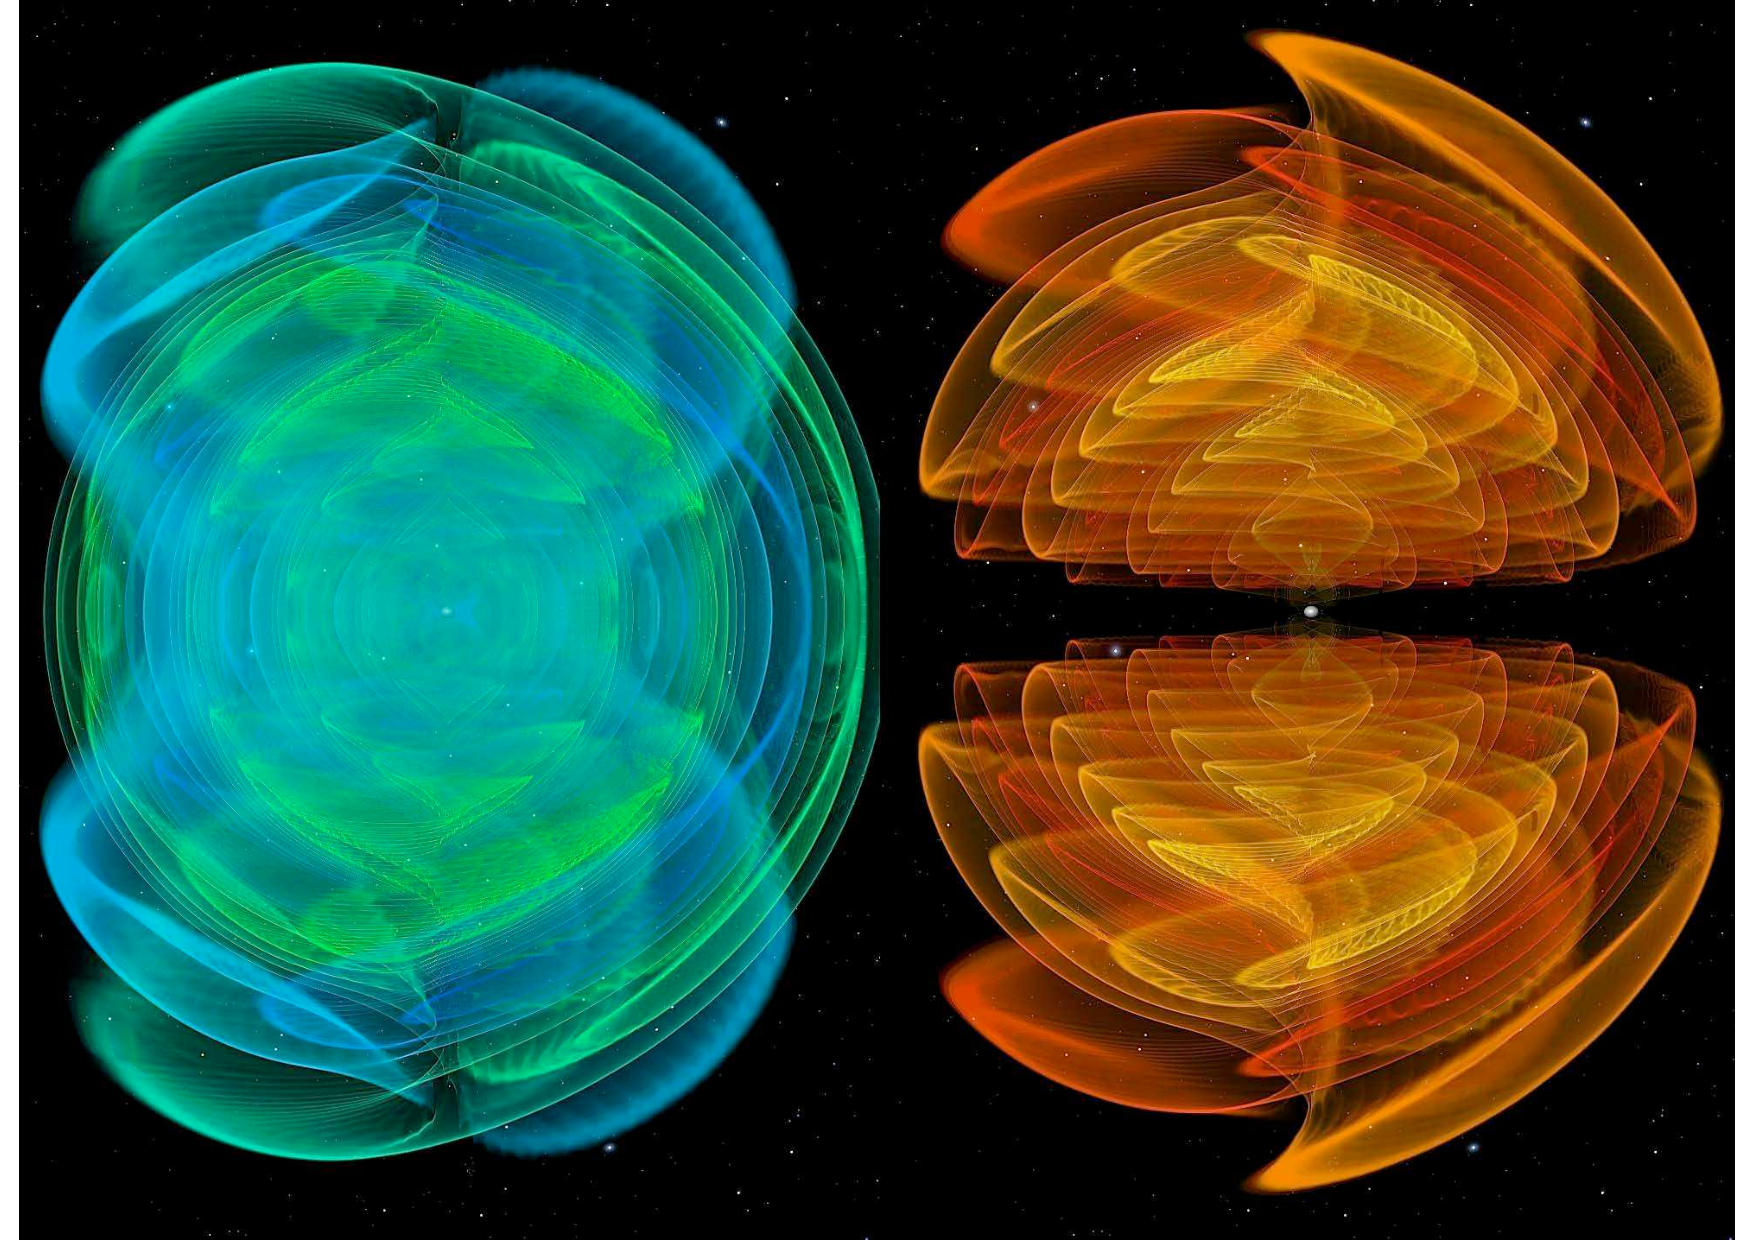
\includegraphics[width=0.88\linewidth,height=0.48\textheight,keepaspectratio]{../figs/pdf/en/fig-08-06.pdf}

% DOCX paragraph 1257
\caption{\emph{Gravitational waves produced by the merger of a binary system of black
holes. © M. Koppitz / C. Reisswig / LR.}}\label{fig:08-06}
\end{figure}

% DOCX paragraph 1258
At the moment of the coalescence, a single \emph{apparent horizon} surrounds and
encompasses the two, still detached, black holes\textsuperscript{\hyperlink{note:08-05}{5}}. The formation of a
common and all-embracing apparent horizon takes place when the two black holes are so
close to each other that their respective horizons are about to touch. Because of the
appearance of this common horizon, a hypothetical external observer would never ``see''
the two black holes touch each other (obviously, I refer to the regions \emph{close} to
the horizons since the latter are not visible by definition). This explains the
enigmatic title of this section, which jokingly summarises the whole evolution process:
1 (black hole) + 1 (black hole) = 1 (new black hole).

% DOCX paragraph 1261
\section{The Perfect Sources Of Energy}\label{sec:08-energy}

% DOCX paragraph 1263
Interestingly, the new black hole produced by the merger will have a mass comparable to
the sum of those of the two initial black holes but a little smaller. The difference is
lost in gravitational waves since the energy they carry is completely equivalent to a
mass, as the notable Equation (3.2) reminds us. More interestingly, this mass can be a
good fraction of that of the two black holes. For example, in the case of the
GW150914\index{GW150914} event, the LIGO detectors measured the gravitational
waveform of a binary system of two black holes with 36 and 29 solar masses, which
merged, as a result of the coalescence, to produce a new black hole of about 62 solar
masses. The missing part (about three solar masses!) is the mass/energy radiated in the
form of gravitational waves in the last milliseconds. If you do the maths, you will then
find out that the binary system has actually lost 5 percent of its mass in gravitational
waves or, if you like, in distorting the rigid fabric of spacetime around it. The rate
of mass loss depends on the properties of the binary system (mass ratio and spin of the
black holes) and can be as high as 10 percent in the case of maximally rotating black
holes. Now, suppose you think of the energy\index{energy!production efficiency} efficiency of nuclear
fission processes, such as those used in nuclear power plants, as being of the order of
0.1 percent. Then it will immediately become clear that the merger of two black holes
represents the most efficient way to produce energy in the whole universe. This also
explains why these sources are visible billions of light years away.

% DOCX paragraph 1264
This enormous loss of energy provides us with an intriguing science fiction perspective.
Perhaps there will come a day when our civilisation is so advanced it can produce
energy, but not through the collision of heavy atoms, as happens now in nuclear power
plants. But through the collision of microscopic black holes in some
``black-hole\index{black hole!power plant} power plant'' located at a safe distance from us in
interstellar space. Among other things, such a power plant would solve the problem of
waste, simply ``directing'' the products of the collision on a path very far from us.
Something I haven't told you is that the black hole produced by the merger generally
acquires a \emph{recoil velocity} (also referred to as ``kick\index{black hole!recoil velocity (kick)}'').
Hence, if the black hole produced is a charged recoiling black hole, it can easily be
diverted and directed wherever desired using magnetic fields. This is clearly a
science-fiction digression, but it has a correct scientific basis. In any case, don't
try this at home!

% DOCX paragraph 1265
Let's go back to the real, astrophysical black holes. Within general relativity and,
except in very particular situations, the final black hole produced by the coalescence
of a binary system of black holes is of the Kerr type, therefore rotating. The rate of
rotation and the direction of the spin vector depends on the initial properties of the
two black holes, particularly on their mass ratio and their spin properties. However,
when it is born, the compact object is not a fully-fledged Kerr black
hole\index{black hole!Kerr} but rather a ``perturbed'' Kerr black hole\index{black hole!Kerr}.
What happens at this point is very interesting: the perturbed black hole is able to
``shake off'' all the imperfections related to its violent formation, so that, within a
few milliseconds (at least in the case of a stellar black hole), every perturbation is
radiated away, that is, lost through the emission of gravitational waves. In this way,
the newly formed black hole rapidly settles into its final (also called asymptotic)
configuration. The gravitational-wave signal emitted when this ``shake off'' takes place
has a very special name; it is referred to as the black-hole
\emph{ringdown}\index{black hole!ringdown}. Because it decays exponentially fast, it is a very
short and evanescent signal, not dissimilar from the sound emitted by a bell when it is
gently ``perturbed'' by the clapper.

% DOCX paragraph 1266
It is important to underline that, just as every bell has a specific sound related to
its properties (mass, shape, metallic alloy, etc.), a black hole has a ringdown signal
closely related to its properties, namely mass and spin. Therefore, the ability to
measure the ringdown signal in the coalescence of a binary system of black holes is
essential; it uniquely collects information about the black hole's properties that are
not otherwise accessible. Furthermore, it serves to confirm that the product of the
merger really is a black hole and not something else. Unfortunately, measuring this
signal, whose amplitude is intrinsically evanescent, is anything but easy. Nevertheless,
it has already been done, for example, by LIGO and Virgo with
GW150914\index{GW150914}, and this measurement served to exclude the object produced
by that merger from being a gravastar\index{gravastar}.

% DOCX paragraph 1269
\section{A Formidable Theoretical Challenge}\label{sec:08-numerics}

% DOCX paragraph 1271
Perhaps, at this point, you are wondering: ``But how do we know all of these
things?\emph{''.} Well, we know because we calculated them numerically almost ten years
before the first gravitational-wave signal was detected. Since the 1990s, a large group
of theoretical physicists from all over the world has been developing advanced
algorithms and constructing sophisticated numerical codes capable of exploiting the
powerful resources offered by parallel supercomputers\index{supercomputers}. This effort
has led to the birth of a new branch of physics, known as \emph{numerical
relativity}\index{numerical relativity}, whose purpose is to solve the Einstein equations
numerically (often together with those of relativistic hydrodynamics\index{relativistic!hydrodynamics}
or magnetohydrodynamics) in order to describe, with the highest possible precision, the
evolution of a binary system of black holes or neutron stars. However, this goal is
anything but trivial as the equations of general relativity, which describe the dynamics
of these objects, are among the most complex known, and the presence of strong
nonlinearities and singularities makes finding the solution particularly challenging.
Indeed, for many years the progress in this area of research has been slow, plagued by
repeated failures and frustrations, to the point that in the late 1990s, no one believed
that numerical relativity would ever calculate anything useful.

% DOCX paragraph 1272
This belief gave rise to a famous bet, made between Kip Thorne\index{Thorne, Kip}
(winner of the Nobel Prize in Physics in 2017) and a group of a dozen scientists engaged
in numerical-relativity research, myself included. The subject of the ``bet'' was who
would get a breakthrough first; Kip bet that LIGO would measure the coalescence signal
of a binary system of black holes before we theorists could calculate it through
numerical- relativity simulations. At stake was a bottle of wine. Undoubtedly, Kip's
intent with the bet was to spur us on, and it worked! The first theoretical signals of
gravitational waves produced by a binary system of black holes were calculated
numerically in 2005. And the first experimental signal was measured ten years later, in
2015, with GW150914\index{GW150914}. Kip Thorne\index{Thorne, Kip} sportingly
acknowledged the defeat and even mentioned it in his Nobel lecture held in Stockholm on
8 December 2017.

% DOCX paragraph 1273
Remarkable progress has been made over the past 15 years through analytical calculations
for the early stages of the dynamics of the binary and numerical simulations for the
final stages, which are more nonlinear and difficult to calculate. This progress has led
to binary systems of compact objects now being the best-understood sources of
gravitational waves.

% DOCX paragraph 1274
Let me stress that being able to compute the gravitational-wave signal has a
significance that goes well beyond the ability to solve a difficult mathematical
problem. A theoretical knowledge of the signal is, in fact, essential for the actual
detection of these sources because, although they release enormous amounts of energy in
the form of gravitational waves, they are usually at considerable distances from Earth,
so the amplitude of their gravitational waves is minimal, as mentioned several times
previously.

% DOCX paragraph 1275
Measurements of this type are clearly at the limit of our technology. Therefore, the
detection of gravitational waves represents a real ``challenge'' not only for
experimental physics but also for theoretical physics. When everything is considered,
including the strength of the signal emitted, the distance of the source, detector
noise, etc., the actual signal measured is often comparable to the background noise of
the detectors. Therefore, it is virtually impossible to measure; in technical jargon, we
say that, under these conditions, the
signal-to-noise\index{signal-to-noise ratio}\index{noise!signal-to-noise ratio} ratio is of order unity. However,
if the signal were known a priori, it is in principle possible to ``extract'' it from
the background noise\index{noise!matched filtering} using a technique called \emph{matched}
\emph{filtering}. To get an idea of what this is, imagine you are listening to a very
noisy radio broadcast in which, despite the crackling noise, it is still possible to
distinguish some words. If we knew some basic information, such as the language used,
the topic discussed, the number of voices speaking into the microphone, etc., our brain
would be able to ``extract'' the signal from the noise and reconstruct what is
transmitted almost entirely. What happens with gravitational waves and matched
filters\index{matched filters} is not so different; prior knowledge allows detectors to
reveal the faintest signal. Thus, over 20 years ago, the formidable theoretical
challenge began to calculate, as precisely as possible, the gravitational waveforms
produced by the most common sources (in all their possible configurations) and provide
this information to the scientists working on the signal detection and data analysis. To
date, this challenge has still not been completed. The prior theoretical knowledge of
the signal allows the scientists to compare the experimental signal mixed with the
detector's noise, filter out the latter and, thus, find the gravitational-wave signal,
even in situations of very low signal-to-noise\index{signal-to-noise ratio}\index{noise!signal-to-noise ratio}
ratios.

% DOCX paragraph 1276
It might seem like a simple goal to achieve, but it is not! Despite the huge progress
made since 2005, the solution of the Einstein equations without approximations and
symmetries remains extremely challenging. To the high complexity of the Einstein
equations, one must add that of the equations of hydrodynamics and magnetohydrodynamics,
which are necessary to describe the motion of matter and equally challenging to solve
under realistic conditions. As a result, the set of coupled partial
differential\index{differential!equations} equations that needs to be solved is so large that its
solution is possible only numerically and by exploiting the resources of the most
powerful parallel supercomputers\index{supercomputers}. Despite all of these difficulties
and problems, the solution of which I have dedicated a good part of my career towards,
the prediction of gravitational waves from compact sources has never been as accurate
and precise. All of these efforts have sealed a tremendous synergy between theory and
experiments in the common goal of detecting gravitational waves and have shown how far
we can go when forces combine.

% DOCX paragraph 1279
\section{Closing With Pure Amazement}\label{sec:08-luminosity}

% DOCX paragraph 1281
By now, you must have realised that I can't help but use equations every now and
then~\ldots{} Hence, I will close this section by returning for a moment to Equation
\eqref{eq:08-01} and, in particular, to the expression to the right. I am well aware that what I am
doing now directly contradicts what I have claimed so far; I need your attention focused
on the constants appearing on the right-hand side of Equation \eqref{eq:08-01}. Yes, the very same
constants I have always recommended you ignore because they are not important. I will
actually do more: to make this change of approach clearer, just this once, I will mark
in black the physical constants \emph{c} and \emph{G}, and grey out all the rest. Hence,
for now, the relevant part of Equation \eqref{eq:08-01} reads:

% DOCX paragraph 1283
\begingroup\renewcommand{\theHequation}{8.repeat}\begin{equation}\tag{8.1}\label{eq:08-01-repeat}
L_{GW} \simeq \frac{c^{5}}{G}\textcolor{gray}{\left( \frac{r_{s}}{R} \right)^{2}\left( \frac{v}{v} \right)^{6}\ }
\end{equation}\endgroup

% DOCX paragraph 1285
Now consider a source of gravitational waves with dimensions equal to the corresponding
Schwarzschild radius and which moves at a speed close to that of light, just as happens
when two black holes are about to merge. In this case, we will have that
\emph{r\textsubscript{s}/R} ≃ 1 and \emph{v/c} ≃ 1 so the greyed out parts in Equation
\eqref{eq:08-02} are roughly equal to one, and the equation effectively depends on the constants
only, reducing to:

% DOCX paragraph 1287
\begin{equation}\label{eq:08-02}
L_{GW}\sim\frac{c^{5}}{G}\sim 3.6 \times 10^{48}\ Watt
\end{equation}

% DOCX paragraph 1289
This gravitational-wave luminosity\index{ luminosity!gravitational wave} is quite simply humongous!
Consider for a moment; there are about one hundred billion (i.e.,
10\textsuperscript{11}) galaxies in the universe, and each of them contains one hundred
billion stars (another factor 10\textsuperscript{11}), each with a brightness of
10\textsuperscript{26} Watts. With Equation \eqref{eq:08-02}, we have just discovered that, at the
moment of the merger, a binary system of black holes radiates as much energy as that
emitted, over the same time and in electromagnetic waves, from the entire universe. I
don't know about you, but it leaves me in a state of pure amazement whenever I think
about this~...

% DOCX paragraph 1292
\section{The Complex Dynamics Of Binary Neutron Stars}\label{sec:08-neutron-stars}

% DOCX paragraph 1294
The dynamics of a binary\index{binary system!neutron stars}\index{neutron star!binary (see)} system of neutron stars
has many similarities with those seen in binary black holes and some fundamental
differences. So, let's arrange things in order and return to the classification of the
phases of the dynamics, of which there are generally four: quasi-circular orbiting,
rapid inspiralling, merger and post-merger\index{post-merger}, and collapse and
accretion.

% DOCX paragraph 1295
The quasi-circular orbiting phase is almost identical to that already discussed for
black holes. Both systems can be described with the same equations and treat the
components of the binary as point-like particles.

% DOCX paragraph 1296
The dynamics of the second phase, rapid inspiralling, is also very similar to that seen
for a black-hole system, but not quite the same. Let me explain why. First of all,
neutron stars have a larger size than a black hole of the same mass. For example, we
have seen that a typical neutron star will have a mass of 1.4 solar masses and a radius
of about 12 kilometres, while a black hole with the same mass will have a Schwarzschild
radius of about 4.2 kilometres. So, keeping the mass the same, a binary system of
neutron stars will merge earlier than a binary system of black holes, simply because the
stars will come to ``touch'' when the separation between the two objects is of the order
of 24 kilometres, rather than eight kilometres. Second, because neutron stars are made
of matter, they can be tidally deformed and, therefore, have slightly different
trajectories from black holes with the same mass. The latter point is particularly
important, so I'll try to explain it in more detail. We have seen that a non-uniform
gravitational field (that is, a normal gravitational field) generates tidal
forces\index{tidal forces} that alter deformable objects, such as the mass of water on
the surface of the Earth, which can be raised by the tidal field produced by the
Moon\index{Moon}. A binary system of compact objects generates a non-uniform
gravitational field since the curvature in the region between the two objects is greater
than that in the more distant regions. Consequently, a deformable object placed in this
non-uniform gravitational field will be deformed in shape. Because a black hole
represents the limit in the strength of the gravitational field, it is not deformable.
We express this fact by saying it has a zero tidal deformability coefficient (also
called \emph{Love number}\index{Love!number})\textsuperscript{\hyperlink{note:08-06}{6}}. In other words, we can
assume that a spherical black hole will remain spherical even if placed very close to
another black hole in a binary system. Here is the crucial difference: this is not the
case with a neutron star. If spherical in isolation, a neutron star will assume a
deformed, non-spherical shape in the presence of another neutron star.

% DOCX paragraph 1297
This change in shape is very significant for two different reasons. The first is that it
induces changes in the orbits followed by neutron stars when compared to those followed
by black holes of the same mass. Consequently, and all things being equal, the
gravitational waves produced by neutron stars during the rapid inspiralling phase will
be different from the corresponding gravitational waves produced by black holes. Indeed,
it is exactly this different behaviour that allows us to discern (once the mass is
known) whether the compact object is a black hole or a neutron star\textsuperscript{\hyperlink{note:08-07}{7}}.
The second reason is even more important. The tidal deformability of neutron stars (that
is, how much they can be deformed in a non-uniform gravitational field) depends on their
internal composition. Therefore, in principle, it is possible to determine their
equation of state\index{equation of state} simply by analysing the gravitational waves in the
final stages of their inspiral, the point when the two stars are at their closest, and
the tidal effects are, therefore, most intense. This is exactly what LIGO and Virgo did
for the GW170817\index{GW170817} event, which provided the first experimental
constraints, albeit still quite uncertain, on the tidal deformability of neutron stars.

% DOCX paragraph 1303
\section{A Fatal Battle Against Gravity}\label{sec:08-remnant}

% DOCX paragraph 1305
The dynamics of the third phase, the merger and post-merger\index{post-merger}, is
decidedly different from what we have seen in the case of black holes. When two neutron
stars merge, they generally do not produce a black hole but a particular type of star,
namely, a \emph{hypermassive} neutron star or HMNS\index{HMNS (hypermassive neutron star)}. The adjective
``hypermassive'' derives from the fact that the mass of this object, which is the sum of
the masses of the two initial stars minus that lost through the collision (which we will
talk about later), is above the maximum mass that we have seen exist for neutron stars
(recall Figure 5.6 in Chapter 5). This hypermassive star is in equilibrium but in a very
precarious equilibrium, which it can very easily lose; for this reason, we say it is in
a \emph{metastable equilibrium}\index{equilibrium!metastable}. In essence, the gravitational field
is so intense (don't forget the hypermassive star is almost twice as massive as the
original stars) that it is on the verge of collapsing to a black hole. However, it
manages to avoid the collapse, at least temporarily, by rotating very rapidly and in a
differential\index{differential!rotation} manner, slower in the core and faster in the outer
layers. In other words, the hypermassive star produced by the collision fights a
desperate battle against gravity, establishing a precarious equilibrium in which it
distributes its matter and rotates almost at the maximum possible rate.

% DOCX paragraph 1306
Unfortunately for the star, it cannot maintain this precarious balance for long because
it rotates so rapidly that it is not even axisymmetric. Instead, the star is deformed
and similar to an enormous ``rotating peanut''. In this configuration, however, it loses
energy and angular momentum through the emission of gravitational waves. This loss will
inevitably lead to gravitational collapse\index{gravitational!collapse} to a rotating black hole.
It is not easy to estimate how long the hypermassive star can carry on its battle
against gravity. This very delicate balance depends, in a nonlinear manner, on a series
of factors, such as the mass of the binary, the mass difference between the two neutron
stars, the equation of state, and the intensity of the magnetic field. Only through
numerical simulations is it possible to accurately describe this phase, which is too
dynamic and nonlinear to be approximated with analytical or perturbative treatments.
From these simulations, we have learned that, depending on all the physical conditions
mentioned above, the hypermassive star can survive only tens of milliseconds (in the
case of very high initial masses) or several hundred milliseconds. Generically, however,
a survival time of more than a few seconds seems very difficult, at least for typical
neutron stars, with initial masses of 1.3-1.4 solar masses.

% DOCX paragraph 1307
During its short life, the hypermassive star performs two essential tasks. The first is
to launch large quantities of matter into interstellar space in the form of high energy
winds (a phenomenon we will discuss in more detail later). The second and possibly even
more important task is to emit copious amounts of gravitational waves precisely because
it is very like a rapidly rotating peanut and, therefore, has large deviations from a
spherical shape. This emission of gravitational waves occurs at precise and almost
constant frequencies related to the properties of the hypermassive star (basically the
mass and equation of state). The emission is imprinted on what is called the
\emph{post-merger}\index{post-merger!gravitational-wave spectrum} gravitational-wave
spectrum\index{spectrum!gravitational wave}\emph{,} the distribution of the energy lost in gravitational
waves as a function of their frequency. The features of the post-merger spectrum are not
dissimilar to a fingerprint, so much so that, in principle, it would be sufficient to
observe the main frequencies characterising the spectrum to obtain information on the
``holy grail'' of nuclear physics: the equation of state of matter at nuclear
densities\index{equation of state}.

% DOCX paragraph 1308
Unfortunately, the prospects for the actual observation of this post-merger
\index{post-merger!gravitational-wave spectrum}spectrum are not very good, at least with current interferometric
detectors. This is because the frequency of the gravitational-wave signal, which is
already very high soon before the merger (around 1 kHz), becomes even higher in the
post-merger\index{post-merger} phase, reaching values of about 2-3 kHz. In practice, the
signal measured by the detectors at these frequencies and for sources at typical
distances expected for binary neutron stars is far too weak and dominated by noise. As a
result, interferometers like LIGO and Virgo are effectively ``deaf'' at these
frequencies. Exactly this happened in the case of the GW170817\index{GW170817} event,
which remained visible for the LIGO detectors for some time before the merger, but whose
signal soon disappeared because it was at frequencies too high to be measured.
Fortunately, these bleak prospects will change radically with the construction of
``third-generation'' interferometric detectors, such as the Einstein Telescope and the
Cosmic Explorer\index{Cosmic Explorer}, which are designed to be much more sensitive in the
2-3 kHz region. When these detectors become operative in about 15 years, it will finally
be possible to measure this weak but enormously important high-frequency signal.

% DOCX paragraph 1309
What happens when the battle is lost? Once the hypermassive star has lost too much of
its rotational energy\index{energy!rotational} and has, thus, exhausted its ability to
withstand gravity, it is forced to collapse into a black hole. However, not all of its
matter is absorbed by the event horizon of the resulting black hole. This is possible
because the hypermassive star is relatively large in size and what
collapses\index{gravitational!collapse} to a black hole is only its inner core. When this happens,
the outer parts of the hypermassive star are at a considerable distance from the centre,
up to 15-20 kilometres. Since the event horizon produced has a radius of about eight
kilometres, some of the star's matter ends up on stable orbits and, therefore, is not
captured by the black hole. Well, at least not immediately. At this point, the system
resulting from the collapse of the hypermassive star is composed of a black hole
surrounded by high-density, high-temperature matter orbiting it. This essentially
constitutes a geometrically thick accretion disc, also referred to as an ``accretion
torus\index{accretion disc!torus}''. To get a better idea of what goes on after the merger, you
should visit my web page and look for the section dedicated to the visualisation of the
numerical simulations carried out by my research group. I believe that visualisation is
better than a thousand words to explain what happens in the complex merger of a binary
system of neutron stars~\ldots{}

% DOCX paragraph 1310
As you can imagine, the accretion torus is also not destined to last too long. The
matter in the torus is highly magnetised and subject to instabilities (particularly the
magnetorotational instability\index{instability!magnetorotational}), which trigger its accretion on the
black hole. Hence, a few seconds after its creation, all of the torus matter is absorbed
by the black hole, which remains the only true witness of the entire coalescence process
of a binary system of neutron stars. Once again, therefore, the bizarre arithmetic of
these systems can be summarised as follows: 1 (neutron star) + 1 (neutron star) = 1
(black hole)\textsuperscript{\hyperlink{note:08-08}{8}}.

% DOCX paragraph 1313
\section{A Mystery That Started With The Cold War}\label{sec:08-gamma}

% DOCX paragraph 1315
A very important difference between the merger of binary black holes and binary neutron
stars is that an electromagnetic counterpart\index{electromagnetic counterpart} is generally expected
from the latter. This expectation is quite natural if you think that the merger of
neutron stars amounts essentially to the collision at speeds close to that of light of
two massive and compact concentrations of matter. Almost inevitably, a process of this
type, with the high densities and temperatures it produces, is bound to produce a signal
relating to electromagnetic radiation\index{radiation!electromagnetic}. However, understanding this
signal requires that I tell you about a mystery that began in the 1970s, in the middle
of the Cold War.

% DOCX paragraph 1316
In those years, the two blocs were heavily involved in fierce competition for both
armaments and technological development. For reasons that today seem all too obvious but
back then were not, the two blocs had agreed on a ban on all nuclear bomb tests. In this
context of non-proliferation of nuclear weapons mixed with the general distrust between
the two superpowers, in the 1970s, the United States launched a spy satellite capable of
collecting radiation in the gamma-ray band. This satellite was very different from how
we may imagine it: instead of pointing to the sky, it was permanently pointed towards
Earth, and, in particular, scanning the vast territory of the Soviet Union. The purpose
of this satellite was obvious enough: to reveal the emission of gamma-ray signals
produced in the case of a nuclear explosion. In other words, it was a satellite built to
measure flashes of gamma rays. The paradoxical aspect of this spy story is that the
satellite did not record any terrestrial events because the Soviets stuck to the
nuclear- test ban. At the same time, the satellite was not a total waste of technology.
On the contrary, it recorded a whole series of gamma-ray flashes of great intensity and
clear celestial provenance. Since these results were protected by military secrecy, the
scientific community knew very little about them. Indeed, it took many years for these
observations to be declassified and many more years for the importance of these
mysterious sources of gamma-ray flashes to become evident. In fact, we had to wait until
the early 1990s for astronomical research in this area to be fully developed.

% DOCX paragraph 1317
Today, after about thirty years of observations of the ``gamma-ray sky'' (or gamma-ray
astronomy\index{astronomy!gamma-ray}), we know that alongside galactic and extragalactic
sources, whose properties are known through repeated measurements, there are also two
classes of sources that are as interesting as they are mysterious. First of all,
\emph{episodic} sources, in the sense that they are observed only once and for very
short periods of time. For this reason, they are called \emph{gamma-ray
bursts}\index{gamma-ray bursts} or GRBs\index{GRBs|see{gamma-ray bursts}}. Since these flashes are very
short, episodic, appear without precursors in other bands, and cannot be measured more
than once, the uncertainty about the sources generating them is still high. However, we
do know that they fall into two broad classes: \emph{long} and \emph{short} bursts.
Despite the name, even the long bursts are extremely short, lasting between a couple of
seconds and about a minute. On the other hand, the short bursts have a much shorter
duration, ranging from a fraction of a second up to about two seconds. Of course, it's
not always easy to distinguish short bursts, accounting for about 30 percent of the
total population, from long bursts. However, when you look at the statistics of all
gamma-ray bursts observed so far (roughly 2,300, with a current average of one gamma-ray
burst observed every day), it becomes clear that there are two distinct populations. One
population has an average duration of around 0.3 seconds for the \emph{short} gamma-ray
bursts\index{gamma-ray bursts!short}, and the other of about 30 seconds for the \emph{long}
gamma-ray bursts\index{gamma-ray bursts!long}.

% DOCX paragraph 1318
In both cases, we are dealing with explosive phenomena that release enormous amounts of
energy (of the order of 10\textsuperscript{50}-10\textsuperscript{52} erg) in a matter
of seconds or less. Furthermore, the observations indicate the clear presence of a
collimated jet that propagates at relativistic speeds, producing gamma-ray radiation
during its propagation or when it collides with the interstellar medium. To get an idea
of how enormous the energy\index{energy!production efficiency} released by these objects is, think of it
like this: in a matter of seconds, gamma-ray bursts release an amount of energy equal to
that emitted by all the stars in our galaxy (amounting to trillions) in one whole year!
For precisely this reason, such flashes are visible from enormous distances and even
from the most remote corners of our universe. Considering the energies involved, the
fact they are generated so far away is actually a good thing, as being hit by even one
of these flashes could represent the end for a large part of life on our planet~...

% DOCX paragraph 1319
It will not come as a surprise to learn that there is no shortage --- indeed, there is
an excess --- of theoretical models capable of explaining the phenomenology observed
with gamma-ray bursts in a more or less satisfactory way. Putting aside the most
imaginative and exotic hypotheses, today's scientific community agrees in associating
the long gamma-ray bursts with the implosion of particularly massive stars. In this
scenario, the collapse of the stellar core generates a black hole that accretes matter
from the stellar interior in the form of an accretion disc and launches a
\index{relativistic!jet} jet that is powerful enough to drill through the rest of the star
and to emerge, becoming visible.\textsuperscript{\hyperlink{note:08-09}{9}}

% DOCX paragraph 1320
By the end of the 1980s, a plausible explanation was proposed for the short gamma-ray
burst\index{gamma-ray bursts!short} involving the coalescence of a binary system of neutron
stars.\textsuperscript{\hyperlink{note:08-10}{10}} This hypothesis seemed perfectly reasonable from the
beginning. The timescales associated with the merger of a neutron star binary are
precisely of the order of 0.1-1 seconds, and the binary system has a huge reservoir of
gravitational energy. Even releasing a few percent of this energy would be sufficient to
account for the measured luminosities of short gamma-ray bursts. Notwithstanding the
plausibility of this model, and hundreds of short gamma-ray bursts being observed over
the past thirty years, the confirmation of this hypothesis only came in 2017 and through
an event we have previously discussed: GW170817\index{GW170817}.

% DOCX paragraph 1323
\section{Much More Than Sources Of Gravitational Waves}\label{sec:08-multimessenger}

% DOCX paragraph 1325
I have already mentioned that the gravitational- wave signal from GW17817 stopped
abruptly at the moment of the coalescence between the two stars. However, I have not
mentioned that something amazing happened soon after that. Just 1.74 seconds after it
disappeared from the gravitational-wave channel, GW170817\index{GW170817}
``reappeared'' in the electromagnetic channel as a short gamma-ray burst: GRB
170817A\index{GRB 170817A}\index{gamma-ray bursts!short}! It was possible to put together the
arrival times of the gravitational-wave signal at the two LIGO detectors and consider
that the Virgo detector had not seen the signal, although, in theory, it could have
done. Scientists from the LIGO/Virgo collaboration promptly located the large, but not
huge, region of the sky where the signal came from and which corresponded to
Virgo's\index{Virgo} \emph{blind spot} (i.e., the region it was not sensitive to
at that time).\textsuperscript{\hyperlink{note:08-11}{11}} Hence, a few seconds after the detection of GW170817,
dozens of telescopes and satellites pointed in the direction of origin of the
gravitational-wave signal, looking for some transient event that could be associated
with it. It was certainly not the first time that a similar exer\index{gravitational-wave detector!blind spot}cise
observational drill had been carried out, as agreements and exchange of alerts are in
place between LIGO/Virgo and a series of observatories scattered over the planet, as
well as satellites in orbit. However, the important difference from all the previous
exercises, which up to that time had involved binary systems of black holes and were
inconclusive\textsuperscript{\hyperlink{note:08-12}{12}}, is that this time an electromagnetic
counterpart\index{electromagnetic counterpart}, albeit weak, was found! It was indeed the signal of a
short gamma-ray burst (named for obvious reasons, GRB 170817A) which appeared quite
ordinary except for its brightness, the lowest ever observed in a gamma-ray burst.
Today, we think that there is probably nothing peculiar about GRB 170817A, and the
reason it appeared so weak is largely a result of our position with respect to its
collimated emission. Interestingly, had we not looked carefully for such emissions in
the right place and at the right time, we would probably have ``missed'' it.

% DOCX paragraph 1326
I recall that the observations of gamma-ray bursts, short or long, show the presence of
a collimated jet of gamma-ray radiation, which we ultimately receive on Earth. Similar
to the case of the radio emissions from pulsars, we can observe a gamma-ray burst only
if we are lucky enough and its emission beam intercepts the Earth in its propagation. If
we think of the jet as a very thin cone, a bright gamma-ray burst is measurable if our
telescopes fall within the opening angle of this cone, which is typically less than ten
degrees. Obviously, we do not observe \emph{all} of the gamma-ray
bursts\index{gamma-ray bursts} produced, even if they are relatively close to us. On the
contrary, we can observe \emph{only} those that are ``pointed'' towards Earth, which
amounts to only about one percent of the total. As for GRB 170817A\index{GRB 170817A}
and its enigmatic low luminosity, today, we believe it appeared dim simply because,
given the relative orientation, we were only marginally invested by the emission cone of
the relativistic jet. For this very reason, the signal would, in all probability, have
been missed had we not pointed the best telescopes in that direction when it was
brightest and searched for a smoking gun. It is only thanks to the tenacity of the
astronomers and their desire to find the first electromagnetic
counterpart\index{electromagnetic counterpart} to a gravitational-wave signal that the window of
multi-messenger gravitational-wave astronomy was finally opened. A window whose
importance we have already discussed. More importantly, the detection of GRB 170817A has
undisputedly shown that the hypothesis put forward nearly 30 years before, namely, that
the coalescence of neutron stars produces short gamma-ray bursts, was not only
reasonable but also correct.

% DOCX paragraph 1327
If it is now clear that merging neutron stars produce light in the form of a gamma-ray
burst\index{gamma-ray bursts}, you may still be wondering: ``How is a relativistic
jet\index{relativistic!jet} actually produced in this process?''. This would be an excellent
question! After all, it is by no means obvious how two dense, compact objects colliding
at near the speed of light can produce an intense jet of radiation. Without getting into
specifics, I must admit we don't yet know the answer to this question. However, there
are helpful clues as to how this can happen, which come from numerical simulations, the
only kind that can provide a sufficiently accurate and realistic picture of what happens
under these conditions.

% DOCX paragraph 1328
An example of these simulations, not the most recent but representing the first study of
this kind and performed by my group\textsuperscript{\hyperlink{note:08-13}{13}}, is shown in Figure \ref{fig:08-07}. The
panels illustrate several instants of a numerical simulation of the coalescence of two
\emph{magnetised} neutron stars, that is, two neutron stars with an ultra-strong
magnetic field.

% DOCX paragraph 1330
\begin{figure}[htbp]
\centering
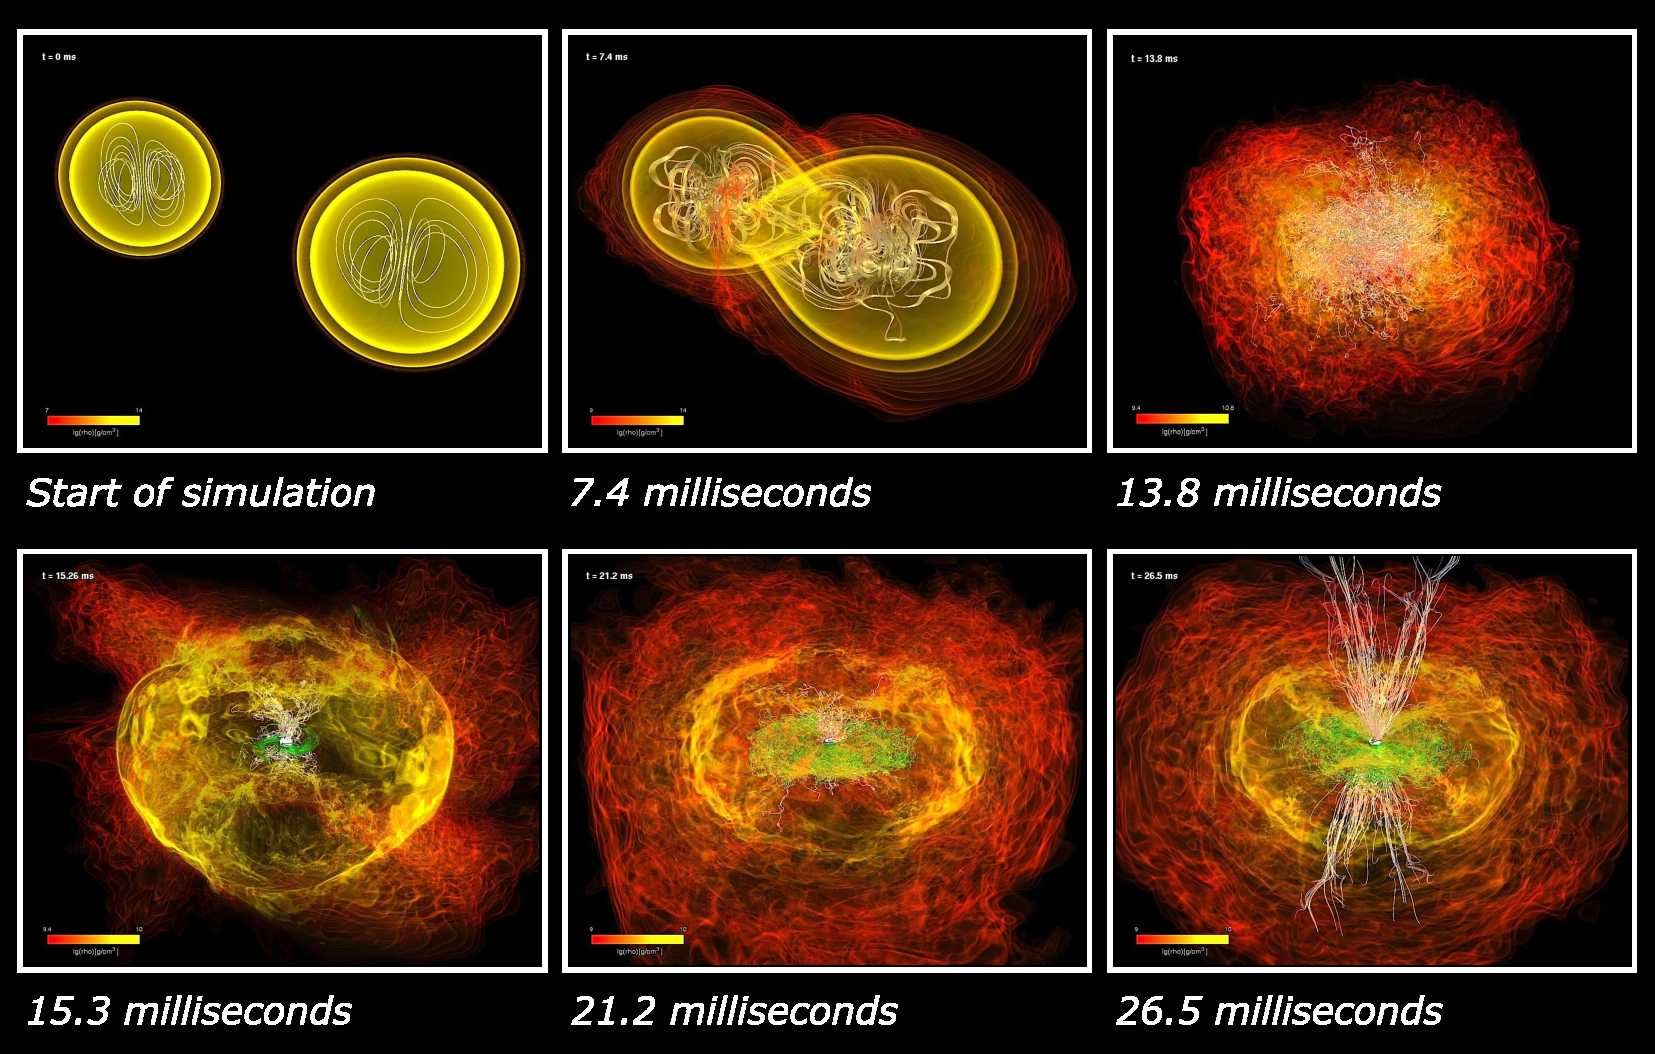
\includegraphics[width=0.88\linewidth,height=0.48\textheight,keepaspectratio]{../figs/pdf/en/fig-08-07.pdf}

% DOCX paragraph 1331
\caption{\emph{Different phases of a numerical simulation of the coalescence of two
magnetised neutron stars. © M. Koppitz/C. Reisswig/LR.}}\label{fig:08-07}
\end{figure}

% DOCX paragraph 1333
The simulations, which were state-of-the-art when performed a decade ago, used a number
of simplifications and did not come without some limitations. For example, although the
geometry of the magnetic field is correct, the velocities of the plasma along the jet
are much slower than those measured with short gamma-ray bursts\index{gamma-ray bursts!short}.
However, the greatest merit of these simulations was to show, \emph{ab initio} (that is,
from first principles), already in 2011, how the presence of a magnetic field is
essential to generate a jet from the coalescence of a binary system of neutron stars. In
other words, through the joint solution of the Einstein equations and those of
relativistic magnetohydrodynamics\index{relativistic!magnetohydrodynamics}, these simulations have taught us
that it is possible to reproduce the phenomenology observed in short gamma-ray bursts,
at least in terms of timescales and energy release, after colliding two magnetised
neutron stars. Alas, ten years later, we are still far from simulating a short gamma-ray
burst in a realistic manner. However, the most modern simulations show increasingly
clearly that binary systems of magnetised neutron stars represent the most promising way
for us to understand how a jet can be produced and move at relativistic speeds towards
us, signalling one of the most catastrophic events in the universe.

% DOCX paragraph 1334
In the hours and days following the first observations of GRB
170817A\index{GRB 170817A}, the electromagnetic signal, which initially was obviously in
the gamma-ray band, continued to be observed at other, gradually lower, frequencies,
passing to the X-ray\index{X-ray!radiation} band, then to the visible band, and finally to
the infrared band. Currently, after several hundred days, it is still possible to detect
an emission from GRB 170817A in the radio band. This type of signal is called
\emph{``afterglow}\index{afterglow}\emph{''} and is produced because, as the source of
emission moves away from the coalescence site, it expands and cools. In this way, the
emission decreases in intensity and its maximum shifts to ever greater wavelengths. Not
very different from what happens with fireworks when the brightness produced by the
explosion fades away and disappears as the cloud of hot gas expands and cools.

% DOCX paragraph 1337
\section{An Explosion Worth Its Weight In Gold}\label{sec:08-gold}

% DOCX paragraph 1339
In addition to the afterglow\index{afterglow}, the emission from short gamma-ray
bursts\index{gamma-ray bursts!short} can be accompanied by a signal in the ultraviolet and optical
bands with a decidedly different origin and which is due to the radioactive decay of
material expelled during the coalescence. In fact, a very robust feature of the merger
of a binary system of neutron stars is that part of the matter that initially
constituted the two stars is ejected to large distances, or, using more technical
jargon, ``lost to spatial infinity''. The reason for this is that part of the matter in
the collision is highly energetic, with speeds higher than the escape velocity from the
gravitational field of the system. The simulations are not yet precise enough to
estimate how much mass is ejected; it depends on a whole series of factors related to
the properties of the binary system. However, it is quite clear that it oscillates
between one-tenth and a few percent of a solar mass. In other words, only a very small
fraction of the system's total mass is actually lost to infinity, but this matter has
enormous importance, as we will see.

% DOCX paragraph 1340
If the idea that a part of the matter of the binary system can be expelled seems obvious
enough, what should happen to this matter is decidedly less obvious. The first
prediction for this was made in 1998 by the astronomers Li-Xin Li\index{Li, Li-Xin} and
Bohdan Paczyński\index{Paczyński, Bohdan}.\textsuperscript{\hyperlink{note:08-14}{14}} Using a simplified model, Li and
Paczyński argued that this matter, which is neutron-rich, i.e., composed of nuclei with
a high number of neutrons (after all, it is the matter that was originally part of the
neutron stars), could undergo radioactive decay. As a result of this decay, it would
generate an electromagnetic emission (quite generically, radioactive matter emits light
when decaying into lighter elements), first in the ultraviolet band and then, over time,
in the visible and infrared bands. This electromagnetic signal, whose genesis is very
different from that of the afterglow\index{afterglow}, was named
\emph{kilonova}\index{kilonova} signal, as it was estimated to be about 1,000 (kilo)
times brighter than that emitted by a \emph{nova}\index{nova}.\textsuperscript{\hyperlink{note:08-15}{15}}
Amazingly, a kilonova signal was observed with GRB 170817A\index{GRB 170817A}, when a
faint decay signal was recorded about 24 hours after the first emission in the gamma-ray
band. At first, this signal emerged with a predominant emission in the blue wavelengths
(for this reason called the \emph{blue kilonova}) \index{kilonova!blue} but then faded
towards longer wavelengths centred around the red (a \emph{red kilonova})
\index{kilonova!red}. This was undoubtedly a beautiful firework, but it was also a strong
confirmation of Li and Paczyński's prediction. The importance of detecting a kilonova
emission is that it provides the final and compelling evidence that a short gamma-ray
burst\index{gamma-ray bursts!short} is intrinsically linked to the coalescence of neutron stars.
Only neutron stars in a merging system of compact objects can eject matter with the high
neutron content necessary to produce and feed the kilonova signal.

% DOCX paragraph 1341
But there is more. The faint kilonova light signal does not only tell us that a very
small portion of the neutron stars can decay radioactively. It also testifies that the
merger process distributes into the interstellar space matter containing heavy and
neutron-rich nuclei. In this way, it solves another problem that has plagued astronomy
for years!

% DOCX paragraph 1342
But let's proceed step by step. Throughout their life, we have seen that stars process
light elements into increasingly heavier elements through a chain that starts from
hydrogen to produce helium, carbon, nitrogen, neon and reaches iron\index{iron}
in the most massive stars. Let me also remind you that ``heavy elements'' are those with
an \index{atomic!mass}\index{mass!atomic}atomic mass greater than that of iron, which is
56. Examples of heavy elements are strontium\index{strontium} (with an atomic mass of
88), caesium (133), europium (152), platinum (195) \index{platinum},
gold\index{gold} (197), and, obviously, uranium (238). Stars can generate heavy
elements only in very small quantities, given that the main chain of nuclear production
is powered by fusion processes that start from hydrogen and end with iron. Furthermore,
when these nuclear processes are exhausted and the stars reach the final stages of their
evolution, all of these elements (be they ``heavy'' or ``light'') remain trapped inside
the stars, with no possibility of being ``scattered'' in the interstellar space. This
simple consideration leads to rather complex questions: ``How could a planet like ours,
which is composed of very heavy elements, such as platinum and uranium, have been
formed? Where did it get its heavy elements from?''.

% DOCX paragraph 1343
An answer to these questions was provided in the early 1960s when it was realised that
massive stars, whose cores contain elements as heavy as iron, can explode in the form of
supernovae and thus distribute these elements in the interstellar space. In addition,
both during the actual supernova\index{supernova} explosion and in the expansion of
the ejected material that follows, \emph{nucleosynthesis} processes can occur, nuclear
processes that synthesise heavy elements from the ashes of the exploded star. Hence,
these studies show that supernovae explosions and the accompanying nucleosynthesis can
generate heavy elements such as those mentioned above. From this, it follows that all of
the matter present on Earth (including us, since we, in small parts, contain
iron\index{iron} and heavy elements) results from the million-year long work of
nucleosynthesis inside the stars. In other words, we are ``sons (and daughters) of the
stars'', well, at least from a nuclear- physics point of view~...

% DOCX paragraph 1344
The problem with this idea, which has emerged only over the last twenty years, is that
this explanation, however plausible and partially correct, is insufficient to explain
the abundance of the heaviest elements measured in the stars around us. In particular,
the calculations estimating how much of these heavy elements are produced in supernova
explosions indicate a much lower abundance than that measured. In other words, there is
too much gold\index{gold} in the universe, more than supernova explosions can
produce~...

% DOCX paragraph 1345
A solution to this problem was first suggested in the mid-1970s when its severity had
not yet become fully apparent. In particular, it was noted that supernova explosions are
not the only processes in which it is possible to expel large quantities of neutron-rich
material and produce heavy elements. It was pointed out that the coalescence of a binary
system containing at least one neutron star is equally effective in this
regard.\textsuperscript{\hyperlink{note:08-16}{16}} Inspired by this suggestion, a whole series of simulations
have been carried out in recent years, which have shown very clearly that the
coalescence of a binary system of neutron stars is indeed ideal from this point of view.
This is because the temperatures and densities reached in the coalescence are so high,
and the matter is already so neutron-rich that the nucleosynthesis of heavy elements is
very efficient. Not only that, the abundance of heavy elements produced in this way is
in good agreement with the observations and depends only weakly on the properties of the
binary system. In essence, the new paradigm that has been developing over the last
decade is that binary systems of neutron stars have the potential to be the optimal
``production site'' for heavy elements in the universe.

% DOCX paragraph 1346
However, all these considerations were only theoretical predictions and nothing more
than the result of complex numerical simulations. For all practical purposes, they were
unsupported by any observational evidence. Fortunately for us, the
GW170817\index{GW170817} event changed all of that! The observation of the
kilonova\index{kilonova} signal has provided confirmation that binary systems of
neutron stars eject substantial quantities of matter into the interstellar space and
that this material can synthesise heavy elements, as predicted by the theoretical
simulations. This confirmation was possible because the light observed in the
kilonova\index{kilonova} signal of GRB 170817A\index{GRB 170817A} showed traces of
the presence of strontium\index{strontium}, an essential heavy element. This was one
of the smoking guns sought for years and the undisputed evidence that heavy elements are
produced in the merger of neutron stars in GW170817!

% DOCX paragraph 1347
If you want to grasp how extraordinary this result is, consider that the quantity of
heavy elements produced in the nucleosynthesis that accompanied
GW170817\index{GW170817} is equal to 16,000 times the mass of the Earth. Even more
impressive is the idea that a good fraction of these heavy elements is represented by
platinum\index{platinum} and gold\index{gold}. And approximately ten ``earth
masses'' (that is, ten times the mass of the Earth) of platinum and gold have been
produced. So, if you are searching for gold, all you have to do is travel in the
direction of GW170817, and you will find more than you can carry back~... These
considerations also bring with them another lesson. We are, indeed, ``children of the
stars'', but also ``children of neutron stars''!

% DOCX paragraph 1348
I want to conclude this \emph{tour de force} on binary neutron stars with a general
consideration. I am fully aware that the amount of information I have given could be
overwhelming, if not confusing. However, I can assure you that these systems are as
impressive to me as they are to you, and I've been working on them for decades. How
could anyone not be amazed to realise that, within only a few hours,
GW170817\index{GW170817} has provided clear answers to questions that have remained
open for decades? With GW170817, we have received confirmation that merging neutron
stars are excellent sources of gravitational waves and emit light in the form of short
gamma-ray bursts\index{gamma-ray bursts!short}. Furthermore, they also eject a few percent of a
solar mass of matter that is particularly rich in neutrons. This matter spreads through
the interstellar medium producing most of the heavy elements present in the universe,
one of which, gold, we humans seem particularly fond of.

% DOCX paragraph 1349
For all of these reasons, the coalescence of a binary system of neutron stars represents
a firework of incredible beauty and a fantastic combination of physical phenomena. All
the fundamental aspects of modern physics converge in this process: the presence of
enormous curvatures of spacetime, the emission of gravitational waves, relativistic
hydrodynamics\index{relativistic!hydrodynamics} and plasma physics, nuclear physics, and the synthesis
of elements. This is why I like to call binary neutron stars \emph{``Einstein's richest
laboratory''}.
